%% 
%% Copyright 2007-2020 Elsevier Ltd
%% 
%% This file is part of the 'Elsarticle Bundle'.
%% ---------------------------------------------
%% 
%% It may be distributed under the conditions of the LaTeX Project Public
%% License, either version 1.2 of this license or (at your option) any
%% later version.  The latest version of this license is in
%%    http://www.latex-project.org/lppl.txt
%% and version 1.2 or later is part of all distributions of LaTeX
%% version 1999/12/01 or later.
%% 
%% The list of all files belonging to the 'Elsarticle Bundle' is
%% given in the file `manifest.txt'.
%% 
%% Template article for Elsevier's document class `elsarticle'
%% with harvard style bibliographic references

\documentclass[preprint,12pt]{elsarticle}
%\documentclass[preprint,12pt,authoryear]{elsarticle}
\usepackage{setspace} \doublespacing
%% Use the option review to obtain double line spacing
%% \documentclass[preprint,review,12pt]{elsarticle}

%% Use the options 1p,twocolumn; 3p; 3p,twocolumn; 5p; or 5p,twocolumn
%% for a journal layout:
%% \documentclass[final,1p,times]{elsarticle}
%% \documentclass[final,1p,times,twocolumn]{elsarticle}
%% \documentclass[final,3p,times]{elsarticle}
%% \documentclass[final,3p,times,twocolumn]{elsarticle}
%% \documentclass[final,5p,times]{elsarticle}
%% \documentclass[final,5p,times,twocolumn]{elsarticle}

%% For including figures, graphicx.sty has been loaded in
%% elsarticle.cls. If you prefer to use the old commands
%% please give \usepackage{epsfig}

%% The amssymb package provides various useful mathematical symbols
\usepackage{amssymb}
\usepackage{subfig}
\usepackage{algorithm2e}
\usepackage{algorithm}
\usepackage{algorithmicx}
\usepackage{kotex}
%% The amsthm package provides extended theorem environments
%% \usepackage{amsthm}

%% The lineno packages adds line numbers. Start line numbering with
%% \begin{linenumbers}, end it with \end{linenumbers}. Or switch it on
%% for the whole article with \linenumbers.
%% \usepackage{lineno}

\journal{Journal}
% of \LaTeX\ Templates}

\begin{document}

\begin{frontmatter}

%% Title, authors and addresses

%% use the tnoteref command within \title for footnotes;
%% use the tnotetext command for theassociated footnote;
%% use the fnref command within \author or \address for footnotes;
%% use the fntext command for theassociated footnote;
%% use the corref command within \author for corresponding author footnotes;
%% use the cortext command for theassociated footnote;
%% use the ead command for the email address,
%% and the form \ead[url] for the home page:
%% \title{Title\tnoteref{label1}}
%% \tnotetext[label1]{}
%% \author{Name\corref{cor1}\fnref{label2}}
%% \ead{email address}
%% \ead[url]{home page}
%% \fntext[label2]{}
%% \cortext[cor1]{}
%% \affiliation{organization={},
%%             addressline={},
%%             city={},
%%             postcode={},
%%             state={},
%%             country={}}
%% \fntext[label3]{}

\title{A Map Matching Algorithm based on Modified Hidden Markov Model considering Time Series Dependency over Larger Time Span}

%% use optional labels to link authors explicitly to addresses:
%% \author[label1,label2]{}
%% \affiliation[label1]{organization={},
%%             addressline={},
%%             city={},
%%             postcode={},
%%             state={},
%%             country={}}
%%
%% \affiliation[label2]{organization={},
%%             addressline={},
%%             city={},
%%             postcode={},
%%             state={},
%%             country={}}
\author{Ha Yoon Song$^{\ast}$ and Jae Ho Lee}
\address{Department of Computer Engineering, Hongik University, 94 Wausan-ro,\\ Mapo-gu, Seoul, South Korea}            
\cortext[mycorrespondingauthor]{Corresponding author}
\ead{hayoon@hongik.ac.kr}

\begin{abstract}
%% Text of abstract
%맵 매칭은 오차가 있는 이동데이터의 실제 위치를 추론하는 기술로, 이동데이터의 핵심 전처리 기술이다. 다양한 맵 매칭 알고리즘 중 은닉 마코브 모델(Hidden Markov Model)을 이용한 맵 매칭이 주목되었다. 하지만 Hidden Markov Model(HMM) 모델은 시계열 데이터의 종속성을 과하게 단순화 시킨다는 문제점이 존재한다. 따라서 다양한 일부 상황들에 대해서 잘못된 매칭 결과를 추론하는 경향을 보인다. 예를 들어 도심지역과 같은 복잡한 도로관계나 이동패턴을 보이는 경우나, 큰 관측 에러와 셈플링 간격 등은 매칭을 더욱 어렵게 만든다. 이에 본 논문은 HMM의 가정을 보완해 새로운 알고리즘, trendHMM 맵 매칭을 제안한다. 해당 알고리즘은 매칭하는 데이터를 포함해 이웃한 데이터들의 움직임을 매칭에 반영하여 더 넓은 범위의 종속성을 고려한다. 그리고 실험을 통해서 다양한 환경의 여러 geopositioning 데이터에 대해서 trendHMM 맵 매칭이 기존의 HMM 맵 매칭보다 더 정확한 결과를 추론함을 보였다.
With the advancement of geopositioning systems and mobile devices, many research with geopositioning data are currently ongoing.
Along the research applications, map matching is a technology that infers the actual position of error-prone trajectory data. It is a core preprocessing technique for trajectory data. Among various map matching algorithms, map matching using Hidden Markov Model (HMM) has gained high attention. However, the HMM model simplifies the dependency of time series data excessively, which leads to inferring incorrect matching results for various situations. 
For example, complex road relationships or movement patterns, such as in urban areas, or serious observation errors and sampling intervals make matching more difficult. In this research, we propose a new algorithm called trendHMM map matching, which complements the assumptions of HMM. 
This algorithm considers a wider range of dependencies of geopositioning data by incorporating the movements of neighboring data into the matching process. For this purpose, the concept of window containing adjacent geoposioning data is introduced. 
Thus trendHMM can utilize relationship among continuous geopositioning data and showed considerable enhancement over HMM-based algorithm.
Through experiments, we demonstrated that trendHMM map matching provides more accurate results than the existing HMM map matching for various environments and geopositioning data sets.
Our trendHMM algorithm shows up to 17.58\% of performance enhancement comparing to HMM based one in terms of Route Mismatch Fraction. 

\end{abstract}

%%Graphical abstract
%\begin{graphicalabstract}
%\includegraphics{grabs}
%\end{graphicalabstract}

%%Research highlights
%\begin{highlights}
%\item Research highlight 1
%\item Research highlight 2
%\end{highlights}

\begin{keyword}
%% keywords here, in the form: keyword \sep keyword

%% PACS codes here, in the form: \PACS code \sep code

%% MSC codes here, in the form: \MSC code \sep code
%% or \MSC[2008] code \sep code (2000 is the default)
%Hidden Markov Model; Map matching; trend;
Map Matching
\sep
Hidden Markov Model
\sep
Geopositioning Data
\sep 
Trajectory Data

\end{keyword}

\end{frontmatter}

%% \linenumbers

%% main text
\section{Introduction}
\label{sec:sec1}
%무선 통신과 geopositioning 기술의 발전으로 인해, 다양한 geopositioning 시스템에서 스마트폰, 차량과 같은 여러 기기에서 위치데이터를 대량으로 수집을 하는 것이 가능해졌다. 그리고 개체의 연속적인 움직임을 주기적인 시계열 형태로 표현할 수가 있다. 다만, 낮은 측정 빈도와 측정 에러 등의 문제로 인해 실제 위치와 차이가 발생하는 경우가 발생할 수 있다. 따라서 적절한 데이터 전처리 과정이 필요하다. 데이터를 전처리하는 과정에서, 대상이 지나간 실제 이동 경로를 추론하기 위한 맵 매칭 기술이 자주 활용된다. 도로 간의 연결 관계를 하나의 그래프로 묘사하고, 특정 시점의 데이터가 어느 간선인지, 즉 어느 도로에 적합할 지 추론하는 방식이다. 다양한 맵 매칭 알고리즘 중에서도 HMM을 이용한 알고리즘이 주목되었다. Newson과 Krum의 연구 \cite{newson2009hidden}에서 처음 등장한 HMM 기반 맵 매칭은 그 성능과 견고함으로 인해 많은 연구에서 활용되었다. 특히, 샘플링 간격이 30초 미만인 데이터에 대해서 성능 뛰어난 것으로 알려져 있다. 하지만 기존의 HMM 기반 맵 매칭 방식은 문제를 과하게 단순화한다. 근본적인 원인으로 $t$ 시점의 데이터는 오직 $t-1$ 시점의 데이터에 대해서만 종속되어 있다는 문제점을 꼽을 수 있다. 따라서 데이터의 오차가 크거나 샘플링 간격이 큰 경우, 혹은 도심 지역과 같이 도로 관계가 복잡한 경우에 기존의 HMM 기반 맵 매칭 방식은 정학하지 않은 결과를 추론한다. 이러한 한계를 극복하고자 \cite{secondHMM1, secondHMM2} 등과 같이 $t-1$ 시점보다 더 이전의 시점을 고려한 high-order HMM을 이용하는 연구도 있었으나, 차원이 늘어날수록 계산 비용이 매우 커지기 때문에 second-order 모델 이상으로 확장하지 못했다. 따라서, 우리는 단순히 차원을 늘리지 않고 데이터 간의 종속성을 확장하기 위하여 여러 데이터들을 묶어 해당 데이터 집합의 움직임 trend를 고려하였다.이에 본 논문은 기존의 HMM 기반 맵 매칭 알고리즘을 보완하여 더 넓은 시점의 종속성을 고려하는 알고리즘인 trendHMM 맵 매칭 알고리즘을 제안한다. 이 알고리즘은 매칭하는 데이터와 이웃한 데이터들을 묶어 더 넓은 범위의 움직임인, "trend"를 고려한다. trend를 고려함으로써 기존 방식이 가지고 있던 종속성 및 차원증가 문제점을 해결할 수가 있었다.다양한 geopositioning 데이터를 이용한 실험을 통해서, trendHMM 맵 매칭 알고리즘이 기존의 HMM 맵 매칭보다 더 정확한 결과를 낼 수 있음을 확인했다. 또한, 대표적인 맵 매칭 알고리즘인 HMM 기반 맵 매칭 알고리즘을 전처리 전/후에 따라 비교하여 trendHMM과 HMM을 매우 정밀하게 비교하였고, 그 결과는 \ref{sec:sec4:sec3}에서 확인할 수 있다. 해당 연구의 주요 내용은 다음과 같다.

Due to advancements in wireless communication and geopositioning technologies, it has become possible to collect a large amount of geolocation data from various devices such as smartphones and vehicles in different geopositioning systems. The continuous movements of objects can be represented in periodic time series form.
However, issues such as low measurement frequency and measurement errors can lead to discrepancies between the actual position and the collected data. Therefore, proper data preprocessing is necessary. During the data preprocessing process, map matching technology is frequently used to infer the actual path taken by the subject. 
This approach involves depicting the connectivity between roads as a graph and inferring which edge, or road, the data at a specific point in time corresponds to. Among various map matching algorithms, those using the Hidden Markov Model (HMM) have gained attention. 
The HMM-based map matching algorithm, first introduced by Newson and Krum \cite{newson2009hidden}, has been widely utilized in research due to its performance and robustness. Particularly, it is known for its excellent performance with data having sampling intervals of less than 30 seconds. However, the existing HMM-based map matching approach oversimplifies the problem. One fundamental issue is that it considers the data at time $t$ to be dependent only on the data at time $t-1$. Therefore, the existing HMM-based map matching approach yields inaccurate results for data with large errors or sampling intervals, as well as for areas with complex road networks such as urban areas. To overcome these limitations, there have been studies utilizing high-order HMMs that consider time points earlier than $t-1$, such as \cite{secondHMM1, secondHMM2}. However, the computational cost significantly increases as the dimensionality increases, preventing the extension of the model beyond second order. Therefore, instead of simply increasing dimensions, we considered the dependencies among various data by grouping multiple data points to account for the movement trend in the dataset, without explicitly expanding the dimensionality. In this research, we propose the trendHMM map matching algorithm, which complements the existing HMM-based map matching algorithm by considering a wider range of dependencies. This algorithm takes into account the "trend," which represents broader movements by grouping the matching data and neighboring data. By considering the trend, we were able to address the issues of dependency and dimensionality increase that the conventional approach had. Through experiments using various geopositioning data, we confirm that the trendHMM map matching algorithm yields more accurate results than the existing HMM map matching approach. 
	Furthermore, we performed a detailed comparison between trendHMM and the well-known HMM-based map matching algorithm, which is a representative map matching algorithm, both with and without preprocessing. This allowed us to make a precise comparison between trendHMM and HMM. The results of this comparison can be found in subsection~\ref{sec:sec4:sec3}. 
	\\The key contributions of this research are as follows: 
	\emph{ 
	\begin{itemize}
		\item It expands the dependency between data by reflecting the movement trend of data.
		\item It demonstrates good performance without the need for data preprocessing, unlike conventional HMM-based algorithms.
		\item It exhibits similar time and space complexity as conventional HMM-based algorithms, but achieves better performance.
	\end{itemize}
}
\emph{The contents of this research paper is as follows: Section~\ref{sec:sec2} discusses about research results related with our topic. 
	In section~\ref{sec:sec3}, a new algorithm developed in this paper, trendHMM, will be explained. As well, we will discuss existing map matching algorithm based on HMM as a basis of our algorithm along with terminology used in the research paper. 
	%% 해당 알고리즘의 한계와 이를 보완한 새로운 알고리즘 trendHMM을 설명한다. 
	Section~\ref{sec:sec4} will show the experimental results, both for HMM-based algorithms and trendHMM algorithm as well as comparison of results of both algorithms.
	%%각각에 대해서 실험을 수행하여 결과값을 비교한다. 마지막으로 
	Final section~\ref{sec:sec5} will conclude this research and discuss about possible future researches.}
	%%에서 연구에 대한 결론과 추후 연구에 대한 방향성을 제시한다.}


%% The Appendices part is started with the command \appendix;
%% appendix sections are then done as normal sections
%% \appendix

%% \section{}
%% \label{}
\section{Related Works}
\label{sec:sec2}
%맵 매칭 survey 논문 \cite{chao2020survey}에 따르면, 맵 매칭 알고리즘은 적용하는 기술의 종류에 따라 크게 네 가지로 분류된다 : Similarity Model, Candidate-Evolving Model, Scoring Model , State-Transition Model.
%Similarity Model은 geometric, topology적으로 가장 가까운 도로를 추론한다. 즉, 이동데이터 모양과 가장 가까운 도로를 매칭한다. 움직이는 대상은 항상 도로 네트워크 위를 움직이고, 한 세그먼트로부터 다른 세그먼트로 도약(leap)할 수 없기 때문에, 측정된 geolocation series는 지도 위에 실제 경로와 유사하다. 위 모델은 일반적으로 높은 효율을 보이지만, 샘플링 간격이 크거나 에러가 큰 경우 혹은 도로가 복잡한 경우에는 낮은 정확성을 보인다.
According to the map matching survey research \cite{chao2020survey}, map matching algorithms can be broadly classified into four categories based on the applied techniques: Similarity Model, Candidate-Evolving Model, Scoring Model, and State-Transition Model.
The Similarity Model infers the closest road geometrically and topologically. In other words, it matches the trajectory data to the road that is closest in terms of shape. Since the moving object always travels on the road network and cannot leap from one segment to another, the measured geolocation series closely resembles the actual path on the map. This model generally demonstrates high efficiency, but it exhibits lower accuracy when dealing with data with large sampling intervals or errors, or in complex road scenarios.

%\emph{본 연구와 관련된 다른 서베이가 존재한다~\cite{jiang2022driving}. 여기에서, 기존의 맵 매칭 알고리즘의 모델들을 분류하고, review하였다. 앞서 말한 Similarity Model, Candidate-Evolving Model, Scoring Model, State-Transition Model 등이  역시 포함되어 있으며, 우리의 연구는 State-Transition Model에 해당한다. 
%이 외에도 맵 매칭과 관련한 다양한 연구 결과들은 다음과 같다.}
\emph{There exists another related survey to our study~\cite{jiang2022driving}. In this survey, the authors classified and reviewed existing map matching algorithms. The previously mentioned Similarity Model, Candidate-Evolving Model, Scoring Model, State-Transition Model, etc., are also included, and our research falls within the State-Transition Model category. In addition to this, various research results related to map matching include the following.}

%\cite{quddus2007current}에선 Similarity Model을 이동데이터의 한 포인트마다 적용하는 point-to-curve와 이동데이터를 묶어 segment를 만든 후 적용하는 curve-to-curve matching \cite{wei2013map}, \cite{zhu2017trajectory}으로 분류 했다. 구체적으로 point-to-curve는 이동데이터를 가장 가까운 도로 네트워크의 edge와 매칭시키며, curve-to-curve는 이동데이터를 묶어 Tr segement를 구성한 뒤 가장 가까운 edge에 매칭시킨다. 가까움을 어떻게 정의 하느냐에 따라 여러 모델이 제안됐으며 대표적인 논문은 \cite{sharma2019map, cui2021hidden}가 있다.
In a research \cite{quddus2007current}, the Similarity Model is further classified into two subcategories: point-to-curve matching, where the model is applied to each point of the trajectory data, and curve-to-curve matching, where the model is applied to segments formed by grouping the trajectory data. This classification is also mentioned in research results such as \cite{wei2013map} and \cite{zhu2017trajectory}.
In point-to-curve matching, each point of the trajectory data is matched with the nearest edge of the road network. On the other hand, in curve-to-curve matching, the trajectory data is grouped to form trajectory (Tr) segments, and then matched with the closest edge. Various models have been proposed based on different definitions of proximity, and notable research in this area include \cite{sharma2019map} and \cite{cui2021hidden}.
%%%%%%%%%% Tr 세그먼트?

%Candidate-Evolving Model은 맵매칭 과정에서 candidate set(particle 또는 hypotheses로 불림)을 유지한다.
%candidate set은 첫번째 Trajectory(Tr) 샘플에 의해 초기화 되고, 기존 후보지들 중 최신 관측값과 거리가 가까운 것들만 남긴다. 알고리즘을 반복해 각 후보지 마다 후보지 조합에 포함된 횟수를 계산할 수 있고, 가장 많이 포함된 후보지들을 모아 segment를 계산해 matching path를 결정한다. 대표적인 모델로 Monte Carlo sampling methods와 Bayesian Inference 방법을 결합한 Particle Filter를 이용한 방법 \cite{wang2016improved,bonnifait2009multi}, Multiple Hypothesis Technique(MHT) \cite{taguchi2018online}를 이용한 방법이 있다.
The Candidate-Evolving Model maintains a candidate set (also known as particles or hypotheses) during the map matching process. The candidate set is initialized by the first trajectory (Tr) sample, and only the candidates that are closest to the latest observation are kept from the existing candidates. By iterating the algorithm, the number of times each candidate is included in the candidate combination can be calculated. The most frequently included candidates are then used to compute segments and determine the matching path.
Prominent models in this category include methods that combine Monte Carlo sampling techniques and Bayesian inference, such as Particle Filter-based approaches \cite{wang2016improved, bonnifait2009multi}, and methods that utilize the Multiple Hypothesis Technique (MHT) \cite{taguchi2018online}. These approaches effectively utilize the candidate set to infer the most likely matching path.

%Scoring Model \cite{quddus2015shortest}과 \cite{sharath2019dynamic}은 특정한 모델을 사용하지 않는다. 각 Tr 세그먼트마다 사전에 정의한 scoring function을 최대로 만드는 후보지들을 찾는다. 특히 \cite{sharath2019dynamic}는 lane-level map matching performance를 달성했다. 먼저, 도로 위의 lane들을 grid 형태로 파티션 한다. 각 time stamp 마다 관측값에 대응되는 후보 grid를 찾고, scoring function을 최대로 만드는 후보를 반환한다. scoring function은 proximity between the grid and trajectory sample 등과 같은 4개의 linear feature을 이용해 결정한다.
The Scoring Model, as described in research such as \cite{quddus2015shortest} and \cite{sharath2019dynamic}, does not rely on a specific model. Instead, it searches for candidate points that maximize a pre-defined scoring function for each Tr segment. In particular, a research shown in \cite{sharath2019dynamic} achieved lane-level map matching performance using this approach.
%In \cite{sharath2019dynamic}, 
The road network is partitioned into grid cells. For each timestamp, the candidate grid cells corresponding to the observed values are identified, and the candidate with the highest scoring function is selected. The scoring function is determined using four linear features, such as the proximity between the grid cell and the trajectory sample.
By utilizing the scoring function, the Scoring Model evaluates and selects the most suitable candidates for each Tr segment, providing a flexible and effective approach for map matching tasks.

%State-Transition Model은 대상이 이동할 수 있는 모든 경로들로 구성된 weighted topological graph를 만든다. 그래프에서 노드는 대상이 특정 순간에 가능한 상태를 의미하고, edge는 다른 timestamp 간 상태의 전이를 의미한다. 따라서 가중치를 가장 크게 만드는 경로를 optimal path로 추론한다. 대표적으로 conditional random field(CRF) 모델 \cite{hunter2013path}, weighted graph transition(WGT) 모델 \cite{hu2016if,lou2009map}, Hidden Markov Model을 이용한 방법이 있다. 세 알고리즘은 유사하나 가중치를 계산하는 방식에 차이가 있으며, 본 논문은 HMM을 이용한 방법에 집중한다.
The State-Transition Model constructs a weighted topological graph consisting of all possible paths that the subject can take. In this graph, nodes represent the possible states of the subject at specific moments, and edges represent transitions between states at different timestamps. The model infers the optimal path by determining the path that maximizes the weights. Notable approaches in this category include the conditional random field (CRF) model \cite{hunter2013path}, the weighted graph transition (WGT) model \cite{hu2016if, lou2009map}, and methods that utilize Hidden Markov Model (HMM).
While these algorithms share similarities, they differ in how they calculate the weights. We focuses on the method that utilizes HMM, which is a popular choice for map matching tasks.

%State-Transition Model 중 하나인 HMM은 가장 널리 쓰이는 방법 중 하나이다. HMM은 Markov chain에서 states를 관측할 수 없으나 측정값으로 추론할 수 있는 경우에 집중한다. 이런 가정은 맵 매칭 문제에 자연스럽다. 각 Tr의 포인트는 관측값으로, 대상의 실제 위치는 관측할 수 없는 상태로 여겨진다. Tr 관측 오류로 인해 측정값 근처의 도로는 잠재적인 실제 대상의 위치(state)이다. 대상이 도로에 실제로 위치했을 때 측정값이 관측될 확률을 방출확률(emission probability)로 표현하고, 대상이 연속적으로 한 후보지에서 연속적인 다음 후보로 이동할 확률을 전이확률로 표현해 가장 높은 확률을 가지는 후보지 조합을 최종 경로로 매칭한다.
HMM (Hidden Markov Model) is one of the most widely used methods in the State-Transition Model for map matching. HMM focuses on cases where the states in a Markov chain cannot be directly observed but can be inferred from the observed measurements. This assumption aligns well with map matching problems, where each point in the trajectory (Tr) is treated as an observed measurement, and the actual position of the subject is considered as an unobserved state.
In HMM, the roads near the measured values are considered potential locations (states) of the subject due to observation errors in the trajectory. The probability of the measured values being observed when the subject is actually located on a road is expressed as emission probability. The probability of the subject transitioning from one candidate location to the next candidate location consecutively is represented as the transition probability. By finding the combination of candidate locations with the highest probability, HMM determines the final matching path.

%HMM을 이용한 맵 매칭은 크게 온라인, 오프라인 모델로 분류된다. 오프라인 모델은 전반적인 Tr 내부의 관계를 파악하기 위해 전체 Tr을 사용하는 방법이다. 샘플링 간격과 관측 에러 변화에 견고한 성능을 보이나 계산 속도가 비효율적이다. 온라인 모델 \cite{goh2012online}에서 처음 제안됐으며, 실시간으로 현재 수집한 데이터까지 묶어 세그먼트를 구성해 맵 매칭한다. 실시간 네비게이션같은 온라인 서비스에 이용하며, 대부분의 온라인 모델은 sliding window를 이용해 매칭을 진행한다. 본 논문은 오프라인 알고리즘에 속한다.
HMM-based map matching can be broadly classified into online and offline models. The offline model uses the entire trajectory (Tr) to understand the overall relationships within it. It demonstrates robust performance against variations in sampling intervals and observation errors but can be computationally inefficient. The online model, first proposed in \cite{goh2012online}, performs map matching by incorporating the data collected in real-time and constructing segments. It is utilized in real-time navigation and similar online services, and most online models employ sliding window techniques for the matching process. The algorithm we will present belongs to offline algorithm.

%최근엔 높은 정확성을 위해 속도,각도,선호도 등 다양한 요소를 이용해 전통적인 HMM를 보완하는 여러 알고리즘이 제안됐다. 에를 들어, \cite{song2012quick,atia2017low,mohamed2016accurate, fu2021online}는 속도제한, road level, difference between vehicle’s heading change and road segments’ heading change 도로들의 heading 변화 간 차이같은 요소를 확률 계산에 포함시켰다. 또한, \cite{fu2021online, reinforce, routechoice}는 휴리스틱 또는 학습을 통해 얻은 driver's travel prerference정보를 고려했다. 
%하지만, 위 모델들은 도로 네트워트가 완벽하다고 가정한다. 도로 네트워크는 Tr이 측정된 시간에 존재하는 모든 도로를 포함하고  표현하지 못한 숨겨진길은 없다고 가정한다. 맵 매칭에서 다양한 요소를 이용할수록 최대한 도로네트워크에 맞춰 해석하는 경향이 있다. 따라서, \cite{wang2013crowdatlas}처럼 맵 매칭을 사용해 네트워크가 잘못 됐을 때 숨겨진 도로를 찾는 map inference 문제에 적합하지 못하다.
Recently, several algorithms have been proposed to enhance traditional HMM-based map matching by incorporating a range of factors such as speed, angle, preference, and more, aiming to achieve higher accuracy. For example, research like \cite{song2012quick,atia2017low,mohamed2016accurate,fu2021online} include factors such as speed limits, road levels, and the difference between the vehicle's heading change and the road segments' heading change in the probability calculations. Additionally, research like \cite{fu2021online,reinforce,routechoice} take into account driver's travel preference information obtained through heuristics or learning.
However, these models assume a perfect road network representation. They assume that the road network includes all roads existing at the time when the trajectory is measured and does not account for any hidden or missing roads. As more factors are considered in map matching, there is a tendency to interpret the data according to the road network as much as possible. Therefore, these models, as shown in \cite{wang2013crowdatlas}, may not be suitable for solving the map inference problem of discovering hidden roads when the network itself is incorrect.

%한편, HMM의 markov property를 극복하기 위해 더 넓은 시간적인 종속성을 고려한 연구도 있었다. 대상의 움직임은 연속적인 시계열이므로 현재 상태와 이전 상태들간의 복잡한 시공간적 관계가 존재한다.즉, Markov property는 맵 매칭 문제를 과도하게 단순화한다. 이를 극복하기 위해 \cite{fu2021online}은 second order로 확장한 HMM 기반 맵 매칭 알고리즘을 제안했고, first-order 방식보다 더 좋은 성능을 보였다. 하지만 \cite{fu2021online}는 계산 효율성 문제로 2차원 이상으로 확장하지 못했다. 본 논문의 알고리즘은 전통적인 HMM 기반 맵 매칭과 동일한 시간복잡도를 가지며 secondHMM 보다 더 넓은 시간 종속성을 고려하는 방법이다.
Indeed, there have been studies that consider a larger temporal dependency to overcome the Markov property in HMM. Since the movement of the target is a continuous time series, there exist complex spatio-temporal relationships between the current state and previous states. In other words, the Markov property overly simplifies the map matching problem. To address this, \cite{fu2021online} proposed a second order HMM-based map matching algorithm, which showed better performance than the first-order approach. However, \cite{fu2021online} did not extend the algorithm beyond two dimensions due to computational efficiency issues. Our aim is to provide an algorithm which maintains the same time complexity as traditional HMM-based map matching but incorporates a larger temporal dependency compared to second order HMM.

%\emph{본 연구와 유사한 목적을 가진 연구 결과가 존재한다~\cite{hu2023amm}. GPS 관측 데이터의 오류를 최소한으로 줄일 수 있는 방법 등을 제안하고 있으며, 본 연구와는 다른 방식으로 모델을 구성하고 있다. 또한 online algorithm을 목표로 하고 있다는 점에서 본 연구와 차별된다.
	%맵 매칭 알고리즘을 기반으로 추가 장비를 이용하여 응용하는 연구 결과도 존재한다 ~\cite{elkholy2023radar}. \cite{elkholy2023radar}에서, 맵 매칭 기술을 응용하는 사례를 보여준다. Autonomous navigation이 요구하는 높은 레벨의 정확도를 위해서 radar/INS integrated position을 맵 매칭 기술을 적용하여 수정한다. }
\emph{There are research results that share similar objectives to our study~\cite{hu2023amm}. It proposes methods to minimize errors in GPS observation data, but its approach to model construction differs from ours. Moreover, its focus on online algorithms is apart from our study.
	There are also research outcomes that utilize additional equipment over map matching algorithms.
	 In \cite{elkholy2023radar}, this research demonstrate cases where map matching technology is applied. It introduced radar/INS integrated techniques with map matching techniques to achieve the high level of accuracy required for autonomous navigation.}
	
%본 논문은 전통적인 HMM 맵매칭을 보완한 통계적인 모델, trendHMM 맵 매칭을 제안한다. 따라서, 다른 맵 매칭 알고리즘보다는 가장 보편적인 맵매칭 알고리즘인 HMM 맵매칭을 중점적으로 비교를 하였다(\ref{sec:sec4:sec3}).직전 시점 뿐만 아니라 더 넓은 시간적 종속성을 고려하기 위해, trendHMM 맵 매칭은 관심있는 포인트 기준으로 몇 개의 데이터들을 묶어 window를 구성한다. window 내부에 대표 포인트들을 뽑아 더 넓게 이동하는 새로운 $Tr_{new}$를 구성한다. $Tr_{new}$를 맵 매칭하는 과정에서 생성된 가중치를 추가적으로 반영해 더 넓은 범위의 움직임, 이동 트렌드를 반영한다. trendHMM은 window의 크기로 시간적 종속성을 조절 할 수 있으며, window 크기가 변화해도 HMM 방식과 동일한 시간 복잡도를 제공한다. 또한, 외부적인 요소 없이 순수한 통계적인 방식의 알고리즘이므로, map inference 문제에 더 좋은 성능을 달성할 수 있으리라 기대한다.
We proposes a statistical model called trendHMM map matching, which complements traditional HMM map matching. 
We primarily focused on comparing the most common map matching algorithm, Hidden Markov Model (HMM) map matching, rather than other map matching algorithms shown in subsection \ref{sec:sec4:sec3}. To consider a larger temporal dependency beyond just the previous timestamp, trendHMM map matching constructs a window by grouping several data points based on the point of interest. Representative points within the window are selected to form a new trajectory $Tr_{new}$ that captures broader movements. During the map matching process of $Tr_{new}$, the generated weights are additionally considered, reflecting the movements and trends over a wider range. The size of the window in trendHMM can be adjusted to control the temporal dependency, and even with varying window sizes, it provides the same time complexity as the HMM approach. Furthermore, as trendHMM is a purely statistical algorithm without external factors, it is expected to achieve better performance in map inference problems.

\section{An Enhanced Version of HMM based Map Matching Algorithm}
\label{sec:sec3}

\emph{
In this section we have to define terminology used in this paper. Then, we will explain basics of existing HMM based map matching algorithm as a basis of our algorithm, with its limitation and point of advancement. The core of this section is subsection~\ref{sec:sec3:sec4} which explains trendHMM algorithm on the basis of previous subsections in this section.
}

\subsection{Terminology}
\label{sec:sec3:sec1}
%이동데이터는 측저된 geopositioning 좌표를 의미하며, trajectory는 이동데이터의 시계열이다.
%각 geopositioning 좌표는 경도, 위도, 타임스탬프를 나타내며, 측정 장비로 인해 실제 위치와는 차이가 있다.
%맵 매칭은 trajectory를 전처리하는 핵심 기술로, 도로 간의 연결 관계를 그래프 형태로 표현하고, 각 이동 데이터를 특정 도로에 매칭하여 개체의 실제 위치를 추론하는 기술이다.
%본 논문에서 사용할 개념은 다음과 같다.
Movement data refers to measured geopositioning coordinates, and a trajectory represents the temporal sequence of movement data. Each geopositioning coordinate includes longitude, latitude, and a timestamp, and there may be discrepancies between the measured coordinates and the actual positions due to inherited geopositioning system properties and/or environmental problems. 
%%%%%%%%%%%%%%%% 참고문헌
% GPS error와 관련된 것은 \cite{gpserror}에 설명되어 있다.
Regarding GPS error is described in \cite{gpserror}.

Map matching is a crucial technology for preprocessing trajectories. It involves representing the connectivity between roads in the form of a graph and assigning each movement data point to a specific road segment, thereby inferring the actual location of the object.
The concepts used in this manuscript are as follows.
\begin{itemize}
	\item Geolocation data : It refers to a single geopositioning point. The t-th movement data in the trajectory is denoted as $g(t)$.
	\item Trajectory (Tr) : It is a time series of movement data. It can be represented as $g(1) \rightarrow g(2) \rightarrow ... \rightarrow g(n)$, and can be written as $Tr_n$. Then the number of geolocation data in $Tr_n$, i.e., cardinality of $Tr_n$ is n.
	\item Road Network : It is represented as a graph to depict the connectivity relationship between roads, denoted as $G(V, E)$. Here, $V$ represents the set of nodes, and $E$ represents the set of edges.
	\item Route : It is a time series composed of edges from the Road Network that match the trajectory, denoted as $Tr$.
\end{itemize}

\subsection{Basics on Map Matching based on HMM}
\label{sec:sec3:sec2}
%맵 매칭의 목적은 Tr의 각 이동데이터들을 도로 네트워크의 특정 간선과 매칭하는 것이다.
%HMM은 대상이 그 시점에서 실제로 위치하고 있는 간선은 은닉 상태로, 측정된 위치 포인트는 관측값으로 모델링하여 그림 \ref{fig:1}과 같이 진행된다.
The purpose of map matching is to match each movement data in the trajectory, denoted as $Tr$, with a specific edge in the road network. The HMM proceeds 
%as shown in the Figure \ref{fig:fig1} 
 by modeling the edge where the object is actually located at that point as a hidden state, and modeling the measured location point as an observed value.

%HMM 맵 매칭 알고리즘의 절차는 다음과 같다.
%먼저 한 이동데이터를 중심으로, 반경이 $r$인 원 안에 있는 도로를 해당 데이터의 후보로 선택한다.
%$C_{g(t)}\in E$는 데이터 $g(t)$의 어떤 후보를 의미한다.
%데이터와 후보 간선 사이 최단 거리와, 최단 거리에 위치한 점 $C_{g(t)}.p, C_{g(t+1)}.p$을 이용해 방출확률과 전이확률을 계산한다.
%방출확률은 실제 위치한 도로가 주어졌을 때 관측값이 측정될 확률이다.
%후보 $C_{g(t)}$에 대한 방출확률 $EP$는 수식 \ref{eq:eq1}과 같다.
First, based on a given mobility dataset, roads within a radius of $r$ are selected as candidates for the data point.
$C_{g(t)}\in E$ represents a candidate for the data point $g(t)$.
The emission probabilities and transition probabilities are calculated using the shortest distance between the data point and candidate edges, as well as the points $C_{g(t)}.p$ and $C_{g(t+1)}.p$ located at the shortest distance.
The emission probability represents the probability of observing a measurement given the actual road position.
The emission probability $EP$ for the candidate $C_{g(t)}$ is defined by equation \ref{eq:eq1}.
\begin{equation}\label{eq:eq1}
	EP(C_{g(t)}) = \frac{1}{\sqrt{2\pi}\sigma }\exp^{\frac{-dist^2}{2\sigma}}
\end{equation}
%수식 \ref{eq:eq1}에서 $dist$는 $g(t)$와 $C_{g(t)}.p$ 사이의 거리를 의미하고, $EP$는  $dist$에 대해 평균이 0인 가우시안 분포를 따른다.
%전이확률은 대상이 실제로 $C_{g(t)}$에서 $C_{g(t+1)}$로 이동할 확률이다.
%그림 \ref{fig:fig1}과 같이 $g(t), g(t+1)$ 사이 거리를 $edist$라 하고, $C_{g(t)}.p, C_{g(t+1)}.p$ 사이 도로를 따라 이동한 최단거리를 $spdist$라 하면, 전이확률 $TP$는 수식\ref{eq:eq2}와 같이 계산되며, $spdist$와 $edist$의 차이에 대해 지수분포를 따른다.
In Equation \ref{eq:eq1}, $dist$ represents the distance between $g(t)$ and $C_{g(t)}.p$, and $EP$ follows a Gaussian distribution with zero mean for $dist$.

\begin{figure}[h]
	\centering
	\subfloat[Example of $C_{g(t).p}$]{
		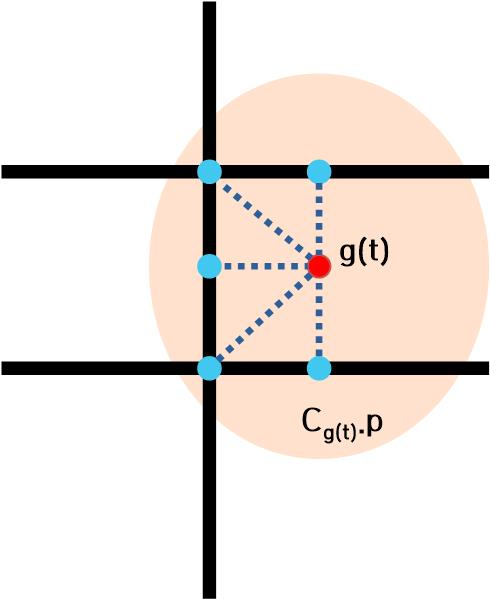
\includegraphics[height=0.25\textheight]{images/fig1a}
	}
	\subfloat[Example of $spdist, edist$ calculated by $g(t), g(t+1)$ and $C_{g(t)}.p,  C_{g(t+1)}.p$]{
		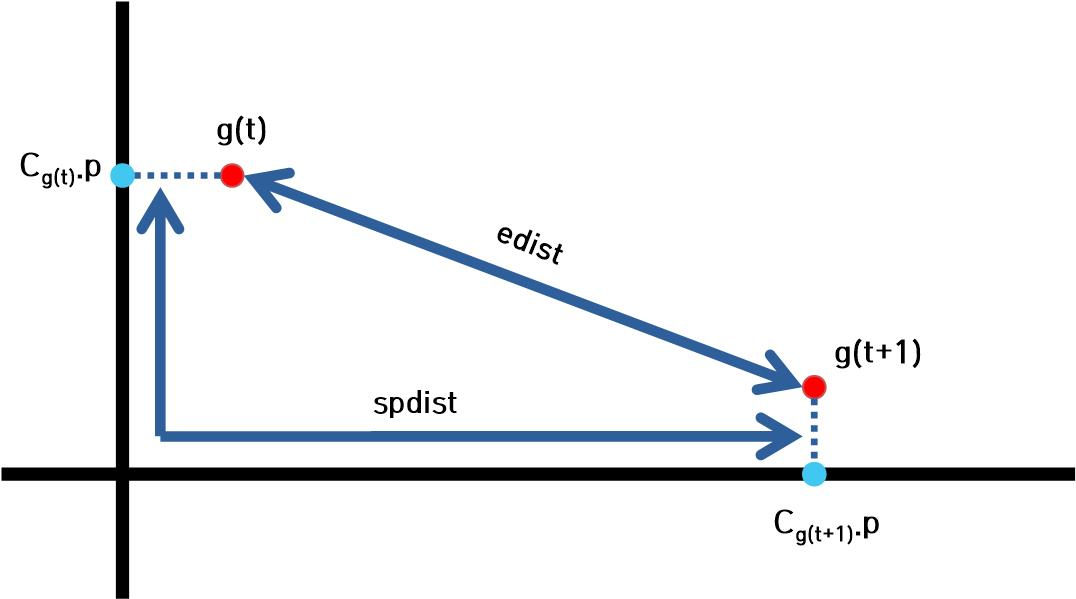
\includegraphics[height=0.25\textheight]{images/fig1b}
	}
	\caption{Typical Operation of Map Matching Algorithm based on HMM}
	\label{fig:fig1}
\end{figure}

The transition probability represents the probability of transitioning from $C_{g(t)}$ to $C_{g(t+1)}$ in reality. As shown in Figure \ref{fig:fig1}, let $edist$ be the distance between $g(t)$ and $g(t+1)$, and let $spdist$ be the shortest distance traveled along the road between $C_{g(t)}.p$ and $C_{g(t+1)}.p$. The transition probability $TP$ is calculated as Equation \ref{eq:eq2}, and it follows an exponential distribution with respect to the difference between $spdist$ and $edist$.

\begin{equation}\label{eq:eq2}
	TP(C_{g(t)},C_{g(t+1)}) = \frac{1}{\beta }\exp ^{-\frac{\left|edist - spdist \right|}{\beta}}
\end{equation}
%알고리즘이 추론하는 실제 경로는 Tr에 대해 수식 \ref{eq:eq4}를 가장 크게 만드는 후보 조합이다.
%수식 \ref{eq:eq3}은 데이터의 각 후보에 대해 방출확률과 전이확률을 계산하는 데 사용될 가중치이다.
%데이터가 후보와 가까울수록, 그리고 $edist$와 $spdist$ 차이가 작을수록 더 큰 값을 갖는다. 이는 Viterbi algorithm\cite{forney1973viterbi}을 이용해 빠르게 계산할 수 있다.
%Viterbi algorithm을 이용한 알고리즘은 \ref{alg:viterbi}와 같다.
The actual path inferred by the algorithm is the combination of candidates that maximizes Equation \ref{eq:eq4} with respect to Tr.
Equation \ref{eq:eq3} represents the weights that will be used to compute emission and transition probabilities for each candidate of the data. The weights are larger for candidates that are closer to the data and have smaller differences between $edist$ and $\label{spdist}$. This can be efficiently computed using the Viterbi algorithm~\cite{forney1973viterbi}.
The algorithm based on the Viterbi algorithm is described in Algorithm \ref{alg:viterbi}.
%알고리즘 \ref{alg:viterbi}에서 Viterbi 알고리즘은 forward, backward 두 단계로 나뉜다. 입력 인자인 $CDS$는 $Tr$의 각 geolocation 데이터에 대한 후보지 집합의 배열(array)이다. 즉, $CDS[t]$는 $g(t)$의 후보지 객체$C_{g(t)}$를 모두 모아 놓은 집합이다. 각 후보지 객체 $C_{g(t)}$는 인스턴스 변수로 edge, prob, prev를 가지며, 알고리즘에서 $C_{g(t)}.variable$으로 표기된다. $C_{g(t)}.edge$는 후보지 객체가 가르키는 도로를 의미한다. $C_{g(t)}.prob$는 $Tr$에서 $g(1)$부터 $g(t)$까지의 최대 $score$(수식 \ref{eq:eq4})값을 저장한다. 따라서, 정해진 $C_{g(t)}$에 대해 아래 수식 \ref{eq:prob}이 성립한다. $C_{g(t)}.prev$는 수식 \ref{eq:prob}에서 값을 최대로 만드는 t-1 후보지를 의미한다.
%\IncMargin{1em}

\singlespacing
\begin{algorithm}[H]
	\KwIn{$ CDS $, array of sets of candidate site objects ($C_{g(t)}$) for all geolocations.}    
	\SetKwFunction{FMain}{forward}
	\SetKwProg{Fn}{Function}{:}{}
	\Fn{\FMain{$CDS$}}{ 
		$L \longleftarrow $ length of $CDS$;\\
		\For{each $C_{g(0)}$ in $CDS[0]$}{
			$C_{g(0)}.prob \longleftarrow 0 $;\\
		}
		\For{$i \gets 0$  \KwTo $L-2$}{
			\For{each $C_{g(i)}$ in $CDS[i]$}{
				$j \longleftarrow i + 1$;\\
				\For{each $C_{g(j)}$ in $CDS[j]$}{
					$ W \longleftarrow TP(C_{g(i)},C_{g(j)}) + EP(C_{g(j)})$;\\
					\If{$C_{g(j)}.prob$ $<$  $C_{g(i)}.prob + W$}{
						$C_{g(j)}.prob \longleftarrow C_{g(i)}.prob + W$;\\
						$C_{g(j)}.prev \longleftarrow C_{g(i)}$;\\
					}
				}
			}
		}
	}
	\textbf{End Function}
	\BlankLine
	\KwIn{$ CDS $, array of candidate site sets for all geolocations.}    
	\KwOut{$ result $, list of street numbers that the algorithm matches to each geolocation.}
	\SetKwFunction{FMain}{backward}
	\SetKwProg{Fn}{Function}{:}{}
	\Fn{\FMain{$CDS$}}{ 
		$result \longleftarrow empty list$;\\
		$L \longleftarrow $ length of $CDS$;\\
		$temp \longleftarrow$ The candidate object in $CDS[L-1]$ with the highest $prob$;\\
		\While{$temp$ is not null}{
			insert $temp.edge$ to $result$;\\
			$temp \longleftarrow temp.prev$;\\
		}
		
		reverse $result$'s order;\\
		\textbf{return} $result$;\\
	}
	\textbf{End Function}
	\caption{An algorithm of HMM map matching with Viterbi}
	\label{alg:viterbi}
\end{algorithm}
\doublespacing

In Algorithm~\ref{alg:viterbi}, the Viterbi algorithm is divided into two stages: forward and backward. The input parameter $CDS$ is an array of candidate sets for each geolocation data in $Tr$. In other words, $CDS[t]$ represents the set of candidate objects $C_{g(t)}$ for $g(t)$. Each candidate object $C_{g(t)}$ has instance variables: $edge$, $prob$, and $prev$, which are denoted as $C_{g(t)}.variable$ in the algorithm. $C_{g(t)}.edge$ represents the road that the candidate object points to. $C_{g(t)}.prob$ stores the maximum $score$ (Equation \ref{eq:eq4}) from $g(1)$ to $g(t)$ in $Tr$. Therefore, for a given $C_{g(t)}$, the following equation (Equation \ref{eq:prob}) holds true. $C_{g(t)}.prev$ refers to the t-1 candidate object that maximizes the value in Equation \ref{eq:prob}.
\begin{equation}\label{eq:eq3}
	W_{hmm}(C_{g(t)},C_{g(t+1)}) =\log ep(C_{g(t+1)}) + \log tp(C_{g(t)},C_{g(t+1)})
\end{equation}
\begin{equation}\label{eq:eq4}
	score(Tr) = \sum_{t=1}^{n-1} W_{hmm}(C_{g(t)},C_{g(t+1)})
\end{equation}
%그리고 알고리즘 \ref{alg:viterbi}에서 forward는 전체 후보지 객체의 prob를 계산하는 함수이다. forward를 실행한 후, $CDS[L-1]$의 후보지 객체 중 가장 큰 prob값이 수식 \ref{eq:eq4}의 $score(Tr)$의 최대값이다. backward는 매칭된 경로를 반환하는 함수이다. $CDS[L-1]$중 가장 큰 prob값을 갖는 후보지 객체부터 시작해, prev를 따라가며 매칭 결과를 반환한다.
In Algorithm \ref{alg:viterbi}, the forward step is a function that computes the probabilities of all candidate objects. After executing the forward step, the candidate object in $CDS[L-1]$ with the highest prob value corresponds to the maximum value of $score(Tr)$ in Equation \ref{eq:eq4}. The backward step is a function that returns the matched path. Starting from the candidate object with the highest prob value in $CDS[L-1]$, it follows the $prev$ pointers to return the matching result of the path.
\begin{equation}\label{eq:prob}
	C_{g(t)}.prob = MAX(C_{g(t-1)}.prob + W_{hmm}(C_{g(t)}))
\end{equation}

\subsection{Limitation of Map Matching based on HMM}
\label{sec:sec3:sec3}
%HMM은 $t$ 시점의 상태의 관측값은 오직 직전 시점 $t-1$의 것과 종속이라 가정한다. 이를 Markov Property라 한다.
%이 가정에는 맵 매칭을 과하게 단순화하는 문제점이 존재하며 이로 인해 잘못된 결과를 도출할 수 있다. 그림 \ref{fig:fig2}이 잘못된 매칭을 보여준다. 빨간색 원 안에 있는 부분은 올바른 경로를 벗어나 잘못 매칭된 것을 보여준다.
%(a)는 샘플링 간격이 크고, 데이터의 에러가 큰 경우이다.
%맵 매칭 과정에서 여러 시점을 고려해야 에러의 영향을 줄일 수 있지만, HMM의 경우 바로 직전 시점만 고려하기 때문에 결과가 난해하다.
%(b)는 도로가 밀집된 도심 지역에서 일어날 수 있는 상황이다. 마찬가지로 데이터 에러의 영향으로 인해 reverse movement 현상이 일어난다.
HMM assumes that the observation at time $t$ depends only on the previous time step $t-1$, which is known as the Markov Property. However, this assumption oversimplifies the map matching process and can lead to incorrect results. Figure \ref{fig:fig2} illustrates incorrect matchings. The area inside the red circle shows incorrect matching, where the path deviates from the correct route.
In Figure \ref{fig:fig2}, (a) represents a case with large sampling intervals and significant data errors. While considering multiple time steps in the map matching process could help mitigate the impact of errors, HMM only considers the immediate previous time step, leading to ambiguous results.
And (b) depicts a situation that can occur in densely populated urban areas. Similarly, due to data errors, a reverse movement can occur.
\begin{figure}
	\centering
	\subfloat[A case with large sampling intervals]{
		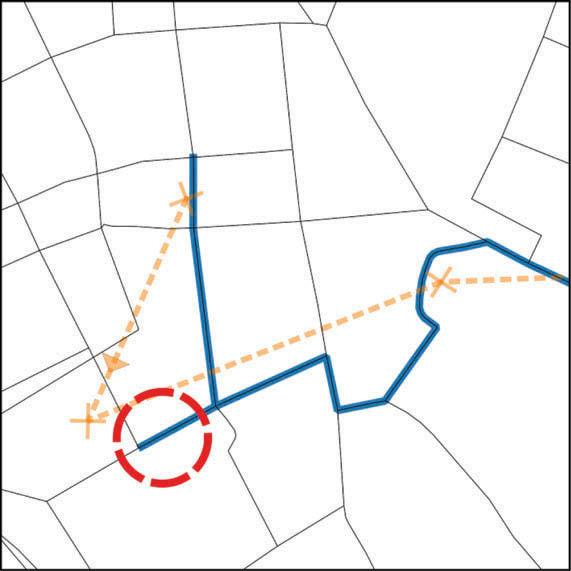
\includegraphics[height=0.25\textheight]{images/fig2a}
	}
	\subfloat[A case with reverse movement]{
		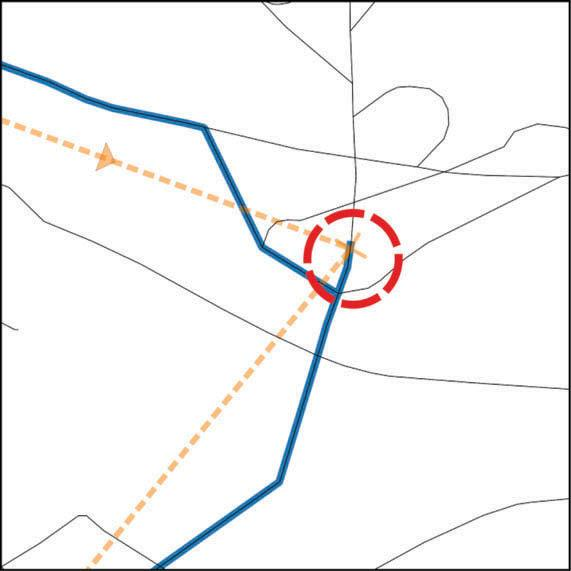
\includegraphics[height=0.25\textheight]{images/fig2b}
	}
	\caption{Example of Erroneous Matching by HMM based Map Matching Algorithm}
	\label{fig:fig2}
\end{figure}

\subsection{Proposed Algorithm: trendHMM Map Matching Algorithm}
\label{sec:sec3:sec4}
\begin{figure}
	\centering
	\subfloat[A movement trend of vehicle]{
		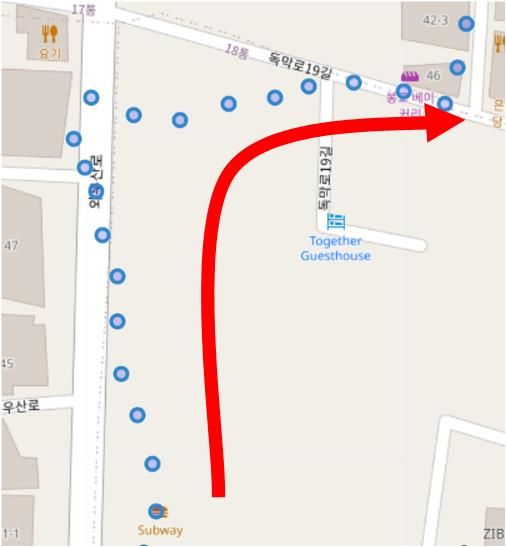
\includegraphics[width=0.25\textheight]{images/fig3a.jpg}
	}
	\subfloat[A movement trend of pedestrian]{
		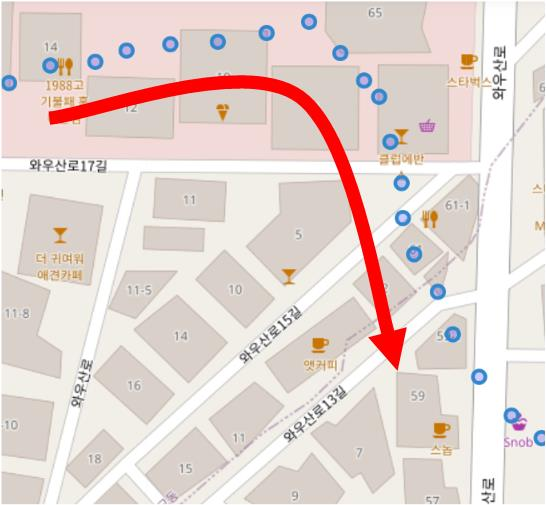
\includegraphics[width=0.25\textheight]{images/fig3b.jpg}
	}
	\caption{Raw Trend Examples: geolocation data (blue dot) and movement trend (red line)}
	\label{fig:fig3}
\end{figure}
%trendHMM의 주요 개념은 다음과 같다.
%$t$ 시점의 이동데이터 $g(t)$는 $t-1$ 시점뿐만 아니라 더 넓은 범위의 이동데이터들과 종속이다.
%특히 $g(t-2),g(t-1),g(t+1),g(t+2)$처럼 $g(t)$와 이웃한 데이터들은 다른 데이터들보다 더 밀접한 관련이 있다.
%이러한 데이터들은 방향, 속도 등 이동과 관련된 특징이 서로 차이가 있으나, 고유한 움직임을 공유한다.
%이웃한 데이터들의 고유한 움직임을 이동 trend라 정의한다. 그림 \ref{fig:fig3}은 트렌드의 예시이다.
%측정된 geopositioning 좌표(파란색 점)들은 관측 에러로 실제 위치와 차이가 있으며, 이동과 관련된 특징이 서로 다르지만 고유한 움직임(빨간색 선)을 공유한다.
%$g(t)$의 실제 위치는 바로 직전 시점의 데이터인 $g(t-1)$뿐만 아니라, 더 넓은 범위의 움직임인 이동 trend에도 크게 영향을 받는다.
%이에 본 논문은 trend를 이용해 전통적인 HMM 모델을 보완한 trendHMM 맵 매칭 알고리즘을 제안한다.
%수식 \ref{eq:eq4}에서 기존 맵 매칭 score를 계산할 때 기존 $W_{hmm}$뿐만 아니라, trend를 고려한 가중치 $W_{trend}$도 이용하고자 한다.
%즉, trendHMM은 다음과 같은 수식 \ref{eq:eq5}를 최대화화하는 후보지 조합을 경로로 추론한다.
The main concepts of trendHMM are as follows.
The movement data $g(t)$ at the time $t$ is dependent on a wider range of movement data as well as the time $t-1$. In particular, neighboring data points such as $g(t-2)$, $g(t-1)$, $g(t+1)$, $g(t+2)$ have a closer relationship with $g(t)$ compared to other data points. Although these neighboring data points may exhibit different characteristics in terms of direction, speed, and other movement-related features, they share a common underlying movement pattern.
These unique movement patterns exhibited by neighboring data points are defined as movement trend. Figure \ref{fig:fig3} provides an example of movement trend. The measured geopositioning coordinates (blue dots) exhibit variations due to observation errors and have different movement-related characteristics. However, they share a common movement trend (red line). The actual location of $g(t)$ is significantly influenced not only by the immediate previous data point, $g(t-1)$ but also by the wider movement trend.
To address this, we proposes a trendHMM map matching algorithm that supplements the traditional HMM model with movement trends.  We introduces a weight $W_{trend}$ that considers the movement trend in addition to the existing weight $W_{hmm}$ combined into  equation \ref{eq:eq4} when calculating the map matching score. In other words, trendHMM aims to infer the path by maximizing the following equation \ref{eq:eq5}, which takes both the traditional HMM score and the movement trend weight into account.
\begin{equation}\label{eq:eq5}
	trend\_score(Tr)= \sum_{t=1}^{t=n-1}( W_{hmm}(C_{g(t)},C_{g(t+1)}) + W_{trend}(C_{g(t+1)}))
\end{equation}
%$W_{trend}$는 trend에 적합한 후보에 더 큰 값을 부여한다.
%후보 $C_{g(t)}$에 대한 $W_{trend}$를 구하는 구체적인 방법은 다음과 같다.
%먼저 그림 \ref{fig:fig4}의 (a)와 같이 $g(t)$를 기준으로 이웃한 데이터 $W$개를 묶어 $window$를 구성하고, $window$ 내부에서 $g(t)$를 포함해 t 이전 시점 데이터들의 중점($lmid$)를 구한다.
$W_{trend}$ assigns a higher value to candidates that fit the movement trend.
The specific method for calculating $W_{trend}$ for candidate $C_{g(t)}$ is as follows. Firstly, create a window by grouping $W$ neighboring data points around $g(t)$ as the reference. This window is constructed to capture the relevant movement trend, as illustrated in Figure \ref{fig:fig4}(a). Within the window, including $g(t)$, calculate the centroid ($lmid$) of the data points from previous time steps.
\begin{figure}
	\centering
	\subfloat[Example of using window (red box) to create $Tr_{new}$, which is composed by $g(out), lmid, g(t), rmid$ (red dot). ]{
		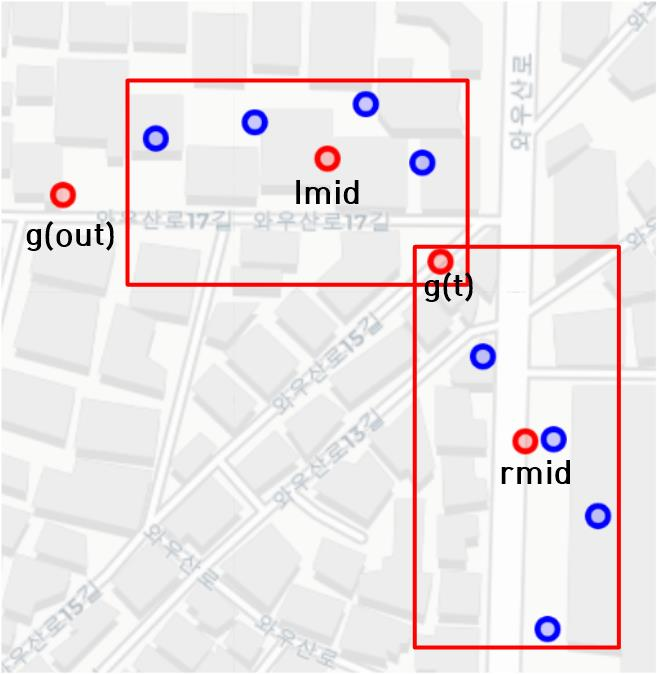
\includegraphics[height=0.25\textheight]{images/fig4a.jpg}
	}
	\subfloat[Example of $Tr_{new}$ and $Tr_{out}$]{
		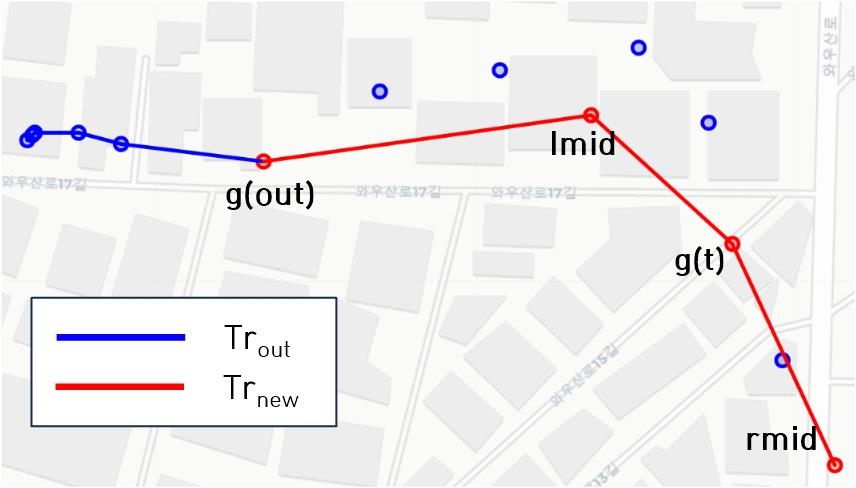
\includegraphics[height=0.25\textheight]{images/fig4b.jpg}
	}
	\caption{Examples of TrendHMM Algorithm Operations}
	\label{fig:fig4}
\end{figure}
%$g(t)$ 이후 시점의 데이터들도 같은 방법으로 중점 $rmid$를 구하고, \ref{fig:fig4}의 (b)와 같이 $g(out)$과 $lmid$, $g(t)$, $rmid$를 연결해 새로운 $Tr_{new}$를 만든다.
%$g(out)$은 window 밖의 데이터로 $out$ 값은 $max(0, t-w+1)$이다.
%중점을 구하기 때문에, $Tr_{new}$는 에러에도 견고하게 trend를 반영한다.
%그림 \ref{fig:fig4}에서 $Tr_{out}$은 기존 trajectory에서 $g(out)$까지의 데이터들로 구성한 trajectory이다.
%다음으로 생성된 $Tr_{new}$, $Tr_{out}$을 이용해 $W_{trend}(C_{g(t)})$를 계산한다. 이는 수식 \ref{eq:eq6}와 같다.
After obtaining the centroid $lmid$ for the data points preceding $g(t)$, the same procedure is applied to the subsequent data points to obtain the centroid $rmid$. Then, as illustrated in Figure \ref{fig:fig4} (b), we connect $g(out)$, $lmid$, $g(t)$, and $rmid$ to create a new trajectory $Tr_{new}$.
$g(out)$ represents the data point outside the window, and its corresponding $out$ value is determined as $max(0, t-w+1)$, \emph{ where w is window size.} By considering the centroids, $Tr_{new}$ incorporates the movement trend more robustly, even in the presence of errors.
In Figure \ref{fig:fig4}, $Tr_{out}$ represents a trajectory constructed from the original trajectory up to $g(out)$.
Finally, the generated $Tr_{new}$ and $Tr_{out}$ are used to calculate $W_{trend}(C_{g(t)})$ according to Equation \ref{eq:eq6}.
\begin{equation} \label{eq:eq6}
	W_{trend}(C_{g(t)})  = \frac{1}{N} max(trend\_score(Tr_{out}) + score(Tr_{new}))
\end{equation}
%수식\ref{eq:eq6}은 $Tr_{out}$에 대해 trendHMM 맵 매칭을 진행하고, $Tr_{new}$에 대해 g(t)의 후보를 특정 $C_{g(t)} $로 고정한 채로 기존 HMM 맵 매칭을 진행한 결과의 최대값이다. 이는 Viterbi 알고리즘으로 빠르게 계산할 수 있다.
%또한, 수식 \ref{eq:eq6}은 기존 $Tr_{out}$의 영향력을 포함해 계산한다. 비터비 알고리즘에 의해 $trend_score(Tr_{out})$은 $W_{trend}(C_{g(t)})$를 구하기 이전에 계산되어 있다.
%$N$은 정규화 파라미터로, 수식 \ref{eq:eq5}에서 각 $W_{hmm}$ 와 $W_{trend}$의 크기를 동일하게 만들기 위해 사용한다.
%수식 \ref{eq:eq6}을 계산할 때 $trend\_score(Tr_{out}$의 총 가중치 개수는 $2out$개, $score(Tr_{new})$는 $3$개이므로, $N$의 값으로는 $2out + 3$을 이용한다.
The equation \ref{eq:eq6} represents the maximum value obtained from conducting trendHMM map matching on $Tr_{out}$ and performing traditional HMM map matching on $Tr_{new}$ while fixing the candidate for $g(t)$ as a specific $C_{g(t)}$. This can be efficiently computed using the Viterbi algorithm.
It's important to note that equation \ref{eq:eq6} incorporates the influence of the original $Tr_{out}$. The trend score $trend\_score(Tr_{out})$ is calculated by the Viterbi algorithm before determining $W_{trend}(C_{g(t)})$.
The normalization parameter $N$ is used to ensure that the magnitudes of each $W_{hmm}$ and $W_{trend}$ in equation \ref{eq:eq5} are equal. 
The value of N can be determined from the equations.
The total number of weights for $trend\_score(Tr_{out})$ is $2\times out$ from Equation \ref{eq:eq5}, and the total number of weights for $score(Tr_{new})$ is $3$ from Equation \ref{eq:prob}. Therefore, the value of $N$ can be set to $2out + 3$ for the calculation of equation \ref{eq:eq6}.
%%%%%%%%%%%%%%% ?????????????????????

%Viterbi 알고리즘을 이용한 trendHMM 알고리즘은 Algorithm \ref{alg:trendViterbi}과 같다.
The trendHMM algorithm using the Viterbi algorithm is described in Algorithm \ref{alg:trendViterbi}.
\begin{algorithm}
	\KwIn{$ CDS $, array of candidate site object (CD) sets for all geolocations.}    
	\SetKwFunction{FMain}{addTrendWeight}
	\SetKwProg{Fn}{Function}{:}{}
	\Fn{\FMain{$t , CDS$}}{
		make candidates array $trendList$ with $g(out),lmid,g(t), rmid$ as shown in Figure \ref{fig:fig4};\\
		calculate $W_{trend}(C_{g(t)})$ using equation \ref{eq:eq6} with $trendList$ and add to $C_{g(t)}.prob$;\\
	}
	\textbf{End Function}
	
	
	\KwIn{$ CDS $, array of candidate site object (CD) sets for all geolocations.}    
	\SetKwFunction{FMain}{trendForward}
	\SetKwProg{Fn}{Function}{:}{}
	\Fn{\FMain{$CDS$}}{ 
		$L \longleftarrow $ length of $CDS$;\\
		\For{each $C_{g(0)}$ in $CDS[0]$}{
			$CD.prob \longleftarrow 0 $;
		} 
		\For{$i \gets 0$  \KwTo $L-2$}{
			addTrendWeight(i, CDS)
			
			\For{each $C_{g(i)}$ in $CDS[i]$}{
				$j \longleftarrow i + 1$
				
				\For{each $C_{g(j)}$ in $CDS[j]$}{
					$ W \longleftarrow TP(C_{g(i)},C_{g(j)}) + EP(C_{g(j)})$;\\
					\If{$C_{g(j)}.prob$ $<$ $C_{g(i)}.prob + W$}{
						$C_{g(j)}.prob \longleftarrow C_{g(i)}.prob + W$;\\
						$C_{g(j)}.prev \longleftarrow C_{g(i)}$;\\
					}
				}
			}
		}
		addTrendWeight(L-1);\\
	}
	
	
	\caption{An algorithm of trendHMM with map matching Viterbi}
	\label{alg:trendViterbi}
\end{algorithm}
%알고리즘 \ref{alg:trendViterbi}에서 trendForward는 trendHMM에 맞게 forward를 수정한 알고리즘이다. addTrendWeight는 trendHMM의 알고리즘대로 trend를 반영해주는 함수이다. 이후 알고리즘 \ref{alg:viterbi}의 backward를 수행해 최종 매칭 경로를 반환한다.
In Algorithm \ref{alg:trendViterbi}, trendForward is an algorithm that modifies the forward step to align with trendHMM. The function addTrendWeight incorporates the trend into the calculation according to the trendHMM algorithm. Afterwards, the backward step of Algorithm \ref{alg:viterbi} is performed to return the final matching path.

%본 논문의 알고리즘은 전통적인 HMM 기반 맵 매칭과 시간복잡도가 동일하다. 한 geolocation 좌표의 평균 후보지 개수를 $C$, $Tr$의 geolocation 개수를 $T$라고 하자. Viterbi 알고리즘에 의해 전통적인 HMM기반 맵 매칭의 시간 복잡도는 $O(TC^2)$ 이다. trendHMM의 경우 한 geolocation당 $Tr_{new}$에 대한 맵 매칭이 추가된다. $Tr_{new}$는 $4$개의 데이터로 구성되어 있으므로, 기존 연산에서 $3$번의 연산이 추가된다. 따라서 trendHMM의 시간복잡도는 $O((3T+T)C^2) = O(4TC^2) = O(TC^2)$이다. 따라서 두 알고리즘의 시간복잡도가 동일하다는 것을 알 수 있다. 또한, HMM과 trendHMM 모두 공간복잡도도 $O(L)$로 동일하다. $L$은 다음 후보지 객체의 개수를 의미한다.
 
	The algorithm proposed in this research has the same time complexity as traditional HMM-based map matching. Let's denote the average number of candidate points for each geolocation coordinate as $C$, and the number of geolocation coordinates in $Tr$ as $T$. The time complexity of traditional HMM-based map matching, determined by the Viterbi algorithm, is $O(TC^2)$.
For trendHMM, each geolocation requires an additional map matching for $Tr_{new}$, which consists of $4$ data points. This means that $3$ additional computations are performed for each geolocation compared to the traditional HMM. However, since $C$ and $T$ remain the same, the overall time complexity of trendHMM remains $O((3T+T)C^2) = O(4TC^2) = O(TC^2)$.
Therefore, we can conclude that the time complexity of both algorithms are the same. 


\emph{For the spatial complexity, both HMM and trendHMM have the same spatial complexity, which is $O(L)$, where $L$ represents the number of candidate spatial objects for the next step.
	Here, $L$ is variable meaning the length of trajectory.
	Regardless of window size, two major points are generated for map matching one point.
	Algorithm~\ref{alg:trendViterbi} generates two more CDS during the process.
	Thus, we can conclude the space complexity of trendHMM algorithm is $O(L + 2L) = O(L)$.
%%	 While executing the algorithm~\ref{alg:trendViterbi}, window size w is constant and is excluded by the definition of big O($\cdot$).
}
%%1. L은 변수입니다. 전체 CDS의 길이니까 Trajectory의 길이를 의미해서 그렇습니다.
%%2. 공간복잡도는 동일하게 O(L)입니다. window size와 관계없이 항상 2개의 중점 좌표를 만들게 되고, 그 과정에서 한 좌표를 맵매칭하는게 추가적으로 2개의 CD를 만들게 됩니다. 모든 좌표를 매칭하는경우, 길이 2L을 추가적으로 연산하니 O(L + 2L) = O(L)입니다.


\section{Experiments}
\label{sec:sec4}
\subsection{Data and Experiment Setup}
\label{sec:sec4:sec1}
%실험에 사용된 데이터셋은 100개의 geopositioning 트랙으로 구성된 대규모 실제 데이터셋으로, 위치는 전 세계 곳곳이다. 데이터셋은 \cite{dataset}에 공개되어있다.
%각 트랙은 map 혹은 map과 올바르게 일치하는 route로 표현된다.
%그리고 일부 트랙에는 맵 매칭 알고리즘에 적용하기 어려울 수도 있는 features로 label되어 있다:
The dataset used in the experiments consists of a large-scale real-world dataset comprising 100 geopositioning tracks, with locations spanning various locations worldwide.The dataset is publicly available in \cite{dataset}. Each track is represented by a map or a route that accurately matches the map.
Additionally, some tracks are labeled with features that may pose challenges for map matching algorithms.
\begin{itemize}
	\item u-turns: the vehicle turned 180$^{\circ}$ and reversed the direction of travel
	\item hives: large numbers of points packed in a small area
	\item loops: the vehicle was traveling in circles
	\item gaps: temporal gaps existing in the track
	\item severe congruence issues: situations where the map and the track are incongruent or dissimilar
\end{itemize}
%또한 연결된 태그가 없는 19개의 고품질 geopositioning 데이터로 형성된 19개의 트랙도 있다.
%트랙의 길이는 5에서 100킬로미터 사이이며, 데이터셋에는 샘플링 속도가 $1Hz$인 총 247,251개의 포인트가 포함되어 있다.
%100개의 트랙의 평균 길이와 평균 길이와 지속 시간은 각각 26.8km와 4950.7초이다. 자세한 내용은 데이터셋 문서인 \cite{dataset}을 참고하기 바란다.
%우리는 10초, 20초, 30초, 60초, 120초의 서로 다른 샘플링 간격으로 원본 데이터를 서브샘플링하여 5개의 데이터셋을 생성하였으며, 각각의 데이터셋에 Douglas-Peucker algorithm~\cite{saalfeld1999topologically} 방식으로 전처리를 한 데이터셋도 추가로 생성하였다.
In addition, in the data sets, there are 19 tracks formed by 19 high-quality geopositioning data points without connected segments. The length of the tracks ranges from 5 to 100 kilometers, and the dataset contains a total of 247,251 points with a sampling rate of 1Hz.
The average length and duration of the 100 tracks are 26.8 km and 4950.7 seconds, respectively. 
More detailed information can be found in the dataset documentation~\cite{dataset}.

We subsampled the original datasets in order to create five different datasets concentrating on sampling intervals rather than one second of original datasets: 10 seconds, 20 seconds, 30 seconds, 60 seconds, and 120 seconds. 
Additionally, we generated preprocessed datasets using the Douglas-Peucker algorithm~\cite{saalfeld1999topologically} on each dataset.

%매칭 정확도는 RMF로 측정되었다.
%이 측정값은 $d_{+}$로 표시되는 false positive 도로 세그먼트의 총 길이와 $d_{-}$로 표시되는 false negative 도로 세그먼트의 총 길이를 계산한다.
%따라서 $d0$이 $d_{+}$의 총 합이라고 했을 때, $RMF$는 map matching error를 $(d_{+} + d_{-}) / d0$의 비율로 정량화하므로 작은 $RMF$ 값이 맵 매칭 결과가 실제 경로와 더 유사함을 나타낸다.
The matching accuracy is measured by the Route Mismatch Fraction (RMF) proposed by Newson and Krumm \cite{newson2009hidden}.
The measured values include the total length of false positive road segments, denoted as $d_{+}$, and the total length of false negative road segments, denoted as $d_{-}$. If we consider $d_0$ as the sum of $d_{+}$, the $RMF$ quantifies the map matching error as the ratio $(d_{+} + d_{-}) / d_0$. A smaller $RMF$ value indicates that the map matching results are more similar to the actual path.

%다음으로, 다양한 샘플링 간격의 geolocation data에 대해서 trendHMM의 효율성을 평가한다. 전통적인 HMM 기반 방법과 (우리의 방법인) trendHMM을 비교하기 위해 각각의 $RMF$ 값을 도출한다.
%실험을 전반에 걸쳐 방정식 \ref{eq:eq1}에서 geopositioning 측정값 표준 편차 $σ$는 두 방식 모두 $10m$로 설정한다.
%transition 확률을 추정하는 데 사용되는 방정식 \ref{eq:eq2}의 scaling factor $β$도 $10m$로 설정되지만 정성적 결과는 \cite{reinforce} 범위에서 유지된다.
%효율성 문제를 위해 각 geopositioning 지점에서 $200m$ 이내에 있는 도로 세그먼트만 검색하여 후보를 구성한다.
%모든 방법은 Python으로 구현하고, 모든 실험은 2개의 Intel Xeon CPU E5-2630 v2 2.60GHz CPU와 64GB RAM으로 진행하였다.
Next, we evaluate the efficiency of trendHMM for geolocation data with various sampling intervals. To compare trendHMM with the traditional HMM-based method, we derive the $RMF$ values for each approach.
Throughout the experiments, we set the geopositioning measurement standard deviation $\sigma$ to $10~ meters$ in Equation \ref{eq:eq1} for both methods. The scaling factor $\beta$ in Equation \ref{eq:eq2}, used for estimating transition probabilities, is also set to $10~meters$, but the qualitative results are maintained within the range reported in \cite{reinforce}.
For efficiency purposes, we construct candidates by searching for road segments within a radius of $200~meters$ from each geopositioning point. All methods are implemented in Python, and the experiments are conducted on two Intel Xeon CPU E5-2630 v2 2.60GHz CPUs with 64GB RAM.

\subsection{Parameter Estimation}
\label{sec:sec4:sec2}
%논문에서 제시한 trendHMM은 추가적으로 윈도우 크기 $W$를 추정해야한다.
%\ref{section:trenHMM}의 알고리즘에 의해 $W$값이 커질수록 고려하는 이동데이터 사이 거리 및 시간 간격이 커진다. 즉, 시간적 종속성의 범위가 커진다.
The trendHMM algorithm proposed in this research requires an additional estimation of the window size, denoted as $W$. According to the algorithm in Section \ref{sec:sec3:sec4}, as the value of $W$ increases, the distance and time interval between the considered movement data points also increase. In other words, the range of temporal dependencies expands.
\begin{figure}
	\centering
	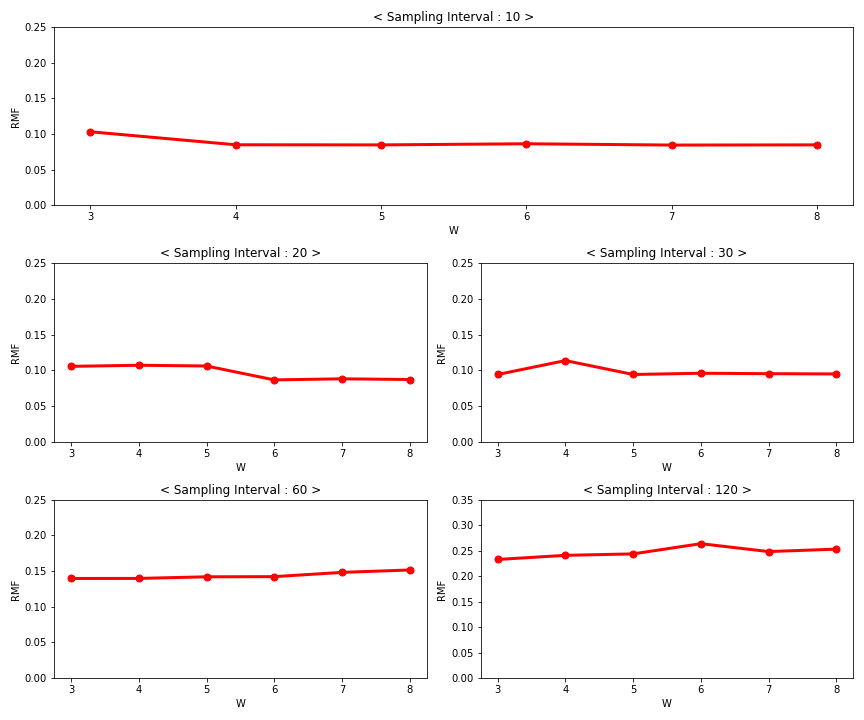
\includegraphics[height=0.99\textwidth]{images/fig5white_0}
	\caption{$RMF$ Values with respect to Window Size W}
	\label{fig:fig5}
\end{figure}

%본 실험에선 다른 샘플링 간격(10s, 20s, 30s, 60s, 120s)으로 만든 데이터에 대해 적절한 $W$ 값을 고르기 위해 아래 그림\ref{fig:fig5}과 같이 값을 변화시켜 가며 실험을 진행했다. 전반적으로 샘플링 간격이 작을 때는 $W$ 값이 클수록 $RMF$ 값이 낮게 나오는 경향이 있는 것을 확인할 수 있다. 다만 샘플링 간격이 클 때는 $W$ 값이 클수록 성능이 낮아지는 것을 확인할 수가 있다. 이동데이터 $g(t)$의 정확한 위치를 추정하기 위해서는 시간과 거리가 가까운 데이터로 구성된 좁은 범위의 이동 trend가 필요하다. 하지만 샘플링 간격이 큰 경우에는, 대략적인 위치 파악은 가능하나 샘플링 간격이 작을 때처럼 정밀하지 못하기 때문에 $W$ 값이 클수록 성능 낮아진다고 볼 수 있다.
In this experiment, we conducted experiments by varying the value of $W$ as shown in Figure \ref{fig:fig5} to select an appropriate $W$ value for the data generated with different sampling intervals (10 sec, 20 sec, 30 sec, 60 sec, 120 sec). Overall, we observed a trend where a higher $W$ value tends to result in lower $RMF$ values when the sampling interval is smaller. However, when the sampling interval is larger, we noticed that a higher $W$ value leads to lower performance. To accurately estimate the precise location of the movement data $g(t)$, a narrow range of movement trend composed of data points with close temporal and spatial proximity is required. However, with larger sampling intervals, although approximate location estimation is still possible, the lack of precision compared to smaller sampling intervals results in lower performance as the value of $W$ increases.

\subsection{Experimental Results}
\label{sec:sec4:sec3}
\begin{figure}
	\centering
	\subfloat[The RMF values of trendHMM with and without Data Preprocessing]{
		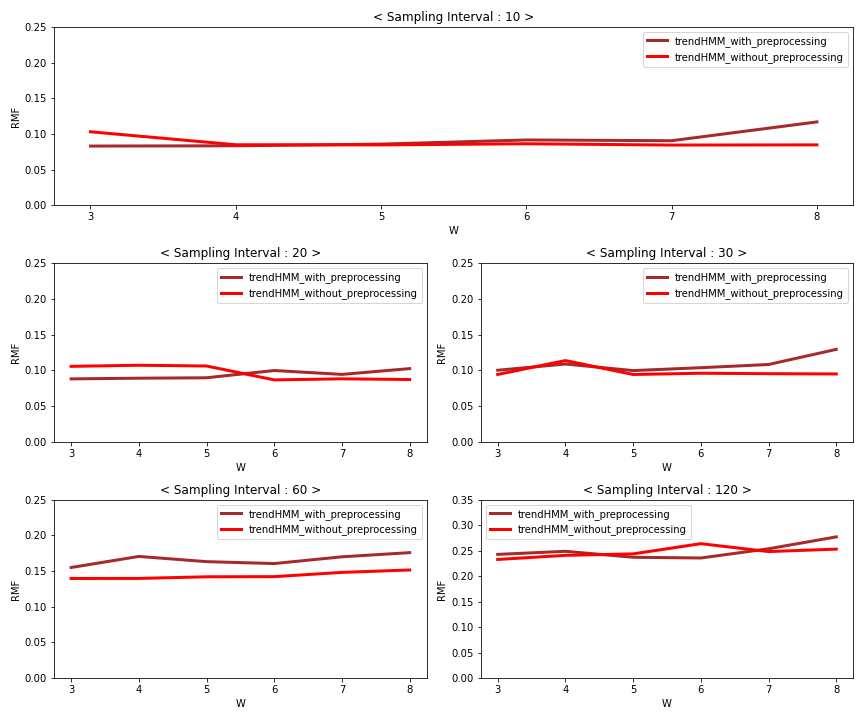
\includegraphics[width=0.7\textheight]{images/trendHMM_unpreprocessing_and_trendHMM_preprocessing_0.png}
	}
\hfill
	\subfloat[The RMF values of HMM with and without Data Preprocessing]{
		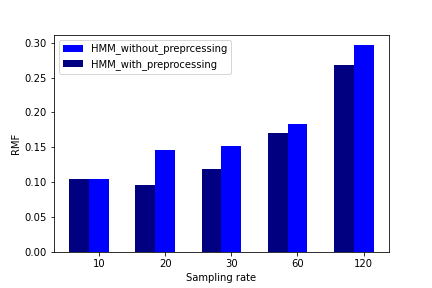
\includegraphics[width=0.5\textheight]{images/HMM_unpreprocessing_and_HMM_preprocessing.png}
	}
	\caption{
		The RMF values of trendHMM and HMM with and without Data Preprocessing}
	\label{fig:fig6}
\end{figure}

\begin{figure}
	\centering
	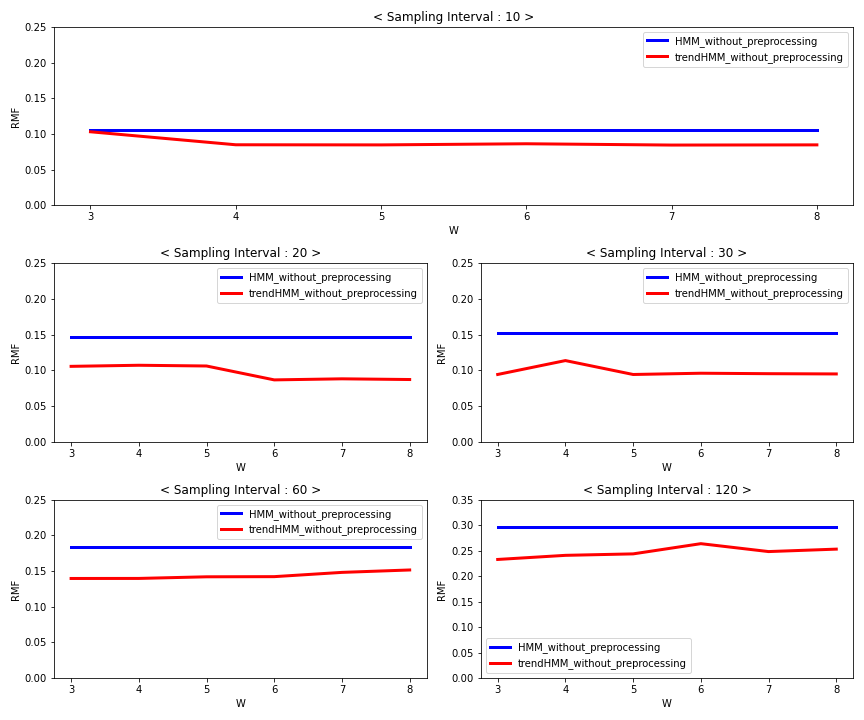
\includegraphics[height=0.99\textwidth]{images/trendHMM_unpreprocessing_and_HMM_unpreprocessing_0.png}
	\caption{The $RMF$ values for trendHMM and HMM, all without Preprocessing}
	\label{fig:fig7}
\end{figure}
\begin{figure}
	\centering
	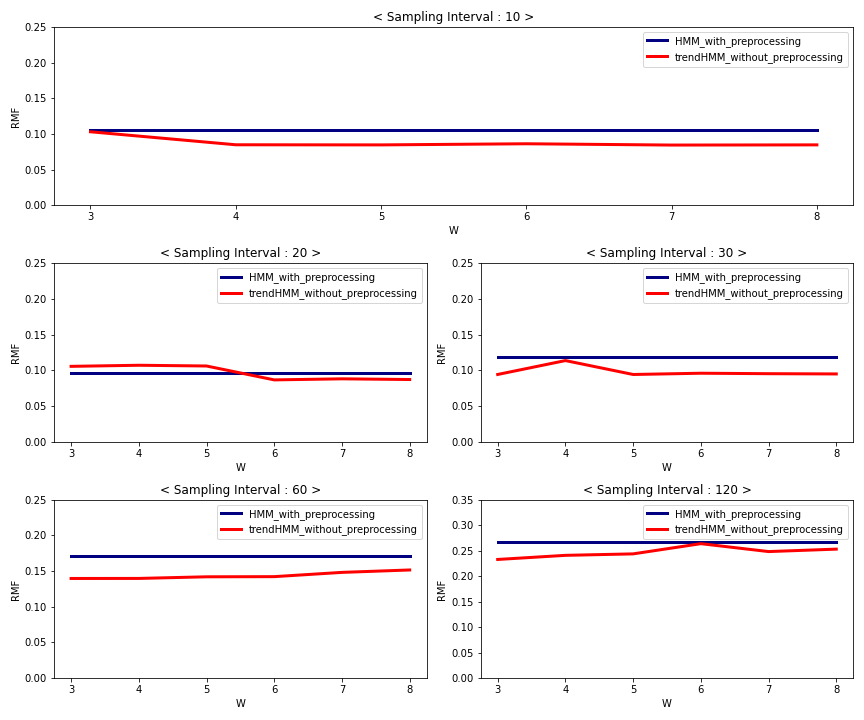
\includegraphics[height=0.99\textwidth]{images/trendHMM_unpreprocessing_and_HMM_preprocessing_0.png}
	\caption{The $RMF$ values for trendHMM without Preprocessing versus HMM with Preprocessing}
	\label{fig:fig8}
\end{figure}
%실험은 trendHMM과 HMM, 데이터 전처리(\cite{saalfeld1999topologically}) 유무로 크게 두 가지의 기준으로 진행을 하였다. 모든 실험에서 데이터 전처리 알고리즘인 Douglas-Peucker Alg.의 파라미터 $epsilon$의 값은 0.001로 고정하였고, $g(t)$ 데이터의 반경 $r$은 0.002로 고정하였고, 이웃한 데이터들의 묶음 개수 $w$는 $\{3, 4, 5, 6, 7, 8\}$로 설정하였다.

%먼저 trendHMM과 HMM의 전처리 유무에 따른 결과값을 비교하였다. 각각의 기본적인 알고리즘은 동일하게 적용되었고, 오직 데이터 전처리 과정이 포함되었는지 안 되었는지의 차이만 있다. 그림 \ref{fig:fig6}에서, (a)는 trendHMM은 without preprocessing이 with preprocessing보다 전반적으로 성능이 더 좋다는 것을 보여주고 있고, (b)는 HMM은 with preprocessing이 without preprocessing보다 성능이 더 좋다는 것을 보여주고 있다. 그림 \ref{fig:fig6}의 (a)에서, 전반적으로 빨간색 라인인 without_preprocessing이 갈색 라인인 with_preprocessing보다 더 낮은 $RMF$ 값을 보여주는데, 이는 trendHMM은 without_preprocessing이 with_preprocessing보다 더 좋은 성능을 보여준다는 의미이다. 반면에 (b)에서는, HMM의 경우 with_preprocessing이 without_preprocessing보다 더 낮은 $RMF$ 값을 보여주고 있다. 즉, trendHMM의 경우 전반적으로 전처리되지 않은 것이 성능이 더 좋게 나왔고, HMM의 경우 전처리한 것이 성능이 더 좋게 나온 것을 확인할 수가 있다.
The experiments were conducted based on two main criteria: trendHMM vs. HMM and the presence or absence of data preprocessing presented by Douglas-Peucker algorithm~\cite{saalfeld1999topologically}. In all experiments, the parameter value $epsilon$ for the Douglas-Peucker algorithm was fixed at 0.001 for data preprocessing. The radius $r$ for the $g(t)$ data was set to 0.002, and the number of neighboring data points to be grouped, denoted as $w$, was set to one of $\{3, 4, 5, 6, 7, 8\}$.
\begin{itemize}
	\item $epsilon$ : The value of the parameter $epsilon$ for the Douglas-Peucker algorithm is 0.001.
	\item $r$ : The value of the radius $r$ for the $g(t)$ data is 0.002.
	\item $w$ : The number of neighboring data points to be grouped, denoted as $w$, is a value from integer set $\{3, 4, 5, 6, 7, 8\}$.
\end{itemize}

Firstly, we compared the results of trendHMM and HMM with and without data preprocessing. Each of the basic algorithms was applied in the same manner, with the only difference being the inclusion or exclusion of the data preprocessing step. In Figure \ref{fig:fig6}, (a) shows that without preprocessing has better overall performance than with preprocessing in trendHMM, and (b) shows that with preprocessing is better in HMM. 
In Figure \ref{fig:fig6} (a), the red line representing "without\_preprocessing" generally exhibits lower $RMF$ values than the brown line representing "with\_preprocessing." This means that trendHMM without preprocessing performs better compared to trendHMM with preprocessing. 
On the other hand, in Figure \ref{fig:fig6} (b), for HMM, "with\_preprocessing" shows lower $RMF$ values than "without\_preprocessing."
In other words, in the case of trendHMM, results without preprocessing are generally better, however, in the case of HMM, it was confirmed that the results with preprocessing are better. 
%다음으로 데이터 전처리가 되지 않은 trendHMM을, 각각의 HMM과 비교하였다. 그림 \ref{fig:fig7}은 without preprocessing HMM과 비교한 것을, 그림 \ref{fig:fig8}는 with preprocessing HMM과 비교한 것을 보여주고 있다. 전반적으로 without preprocessing trendHMM은 each HMM보다 월등한 성능을 보여줌을 확인할 수가 있다.
Next, we compared the non-preprocessed trendHMM with each HMM. Figure \ref{fig:fig7} shows a comparison with the HMM without preprocessing, and Figure \ref{fig:fig8} shows a comparison with the HMM with preprocessing. Overall, it can be confirmed that trendHMM without preprocessing shows superior performance than the cases of HMM with or without preprocessing.

\begin{figure}
	\centering
	\subfloat[	Map with the highest error.]{
		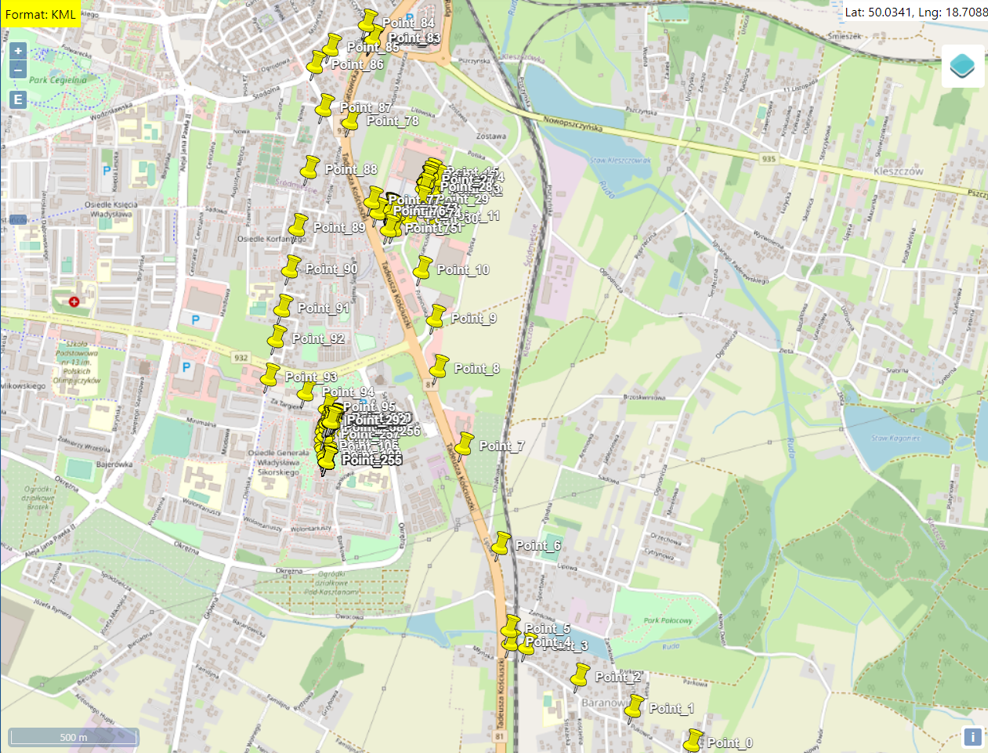
\includegraphics[width=0.5\textheight]{images/track33_20.png}
	}
\hfill
	\subfloat[Map with the second highest error.]{
		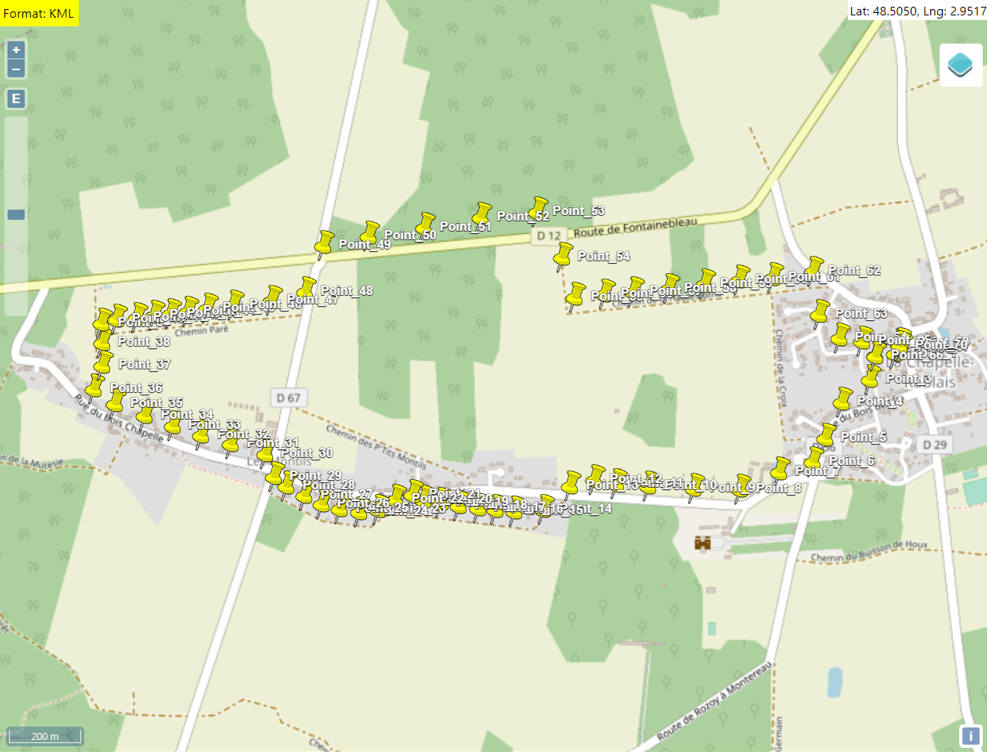
\includegraphics[width=0.5\textheight]{images/track46_20.png}
	}
	\caption{%성능이 낮게 나온 데이터셋의 지도
		A Mapping of the Geopositioning Dataset representing Unexpected Results }
	\label{fig:fig9}
\end{figure}
%다만, trendHMM과 전처리가 적용된 HMM의 그래프에서 샘플링 간격이 20s인 경우, $W$ 값이 $[3, 4, 5]$일 때, trendHMM이 더 낮은 성능이 나왔다. 따라서 그 원인을 파악하기 위하여, 성능이 낮게 나온 일부 데이터를 지도에 그려보았다. 그림 \ref{fig:fig9}을 보면, 한 곳에 오랫동안 머무르는 경우가 해당되는 것을 확인할 수 있다. (a)는 오차가 가장 높게 나타난 지도이며, (b)는 두 번째로 오차가 높게 나타난 지도이다. 아마 데이터 전처리(\cite{saalfeld1999topologically}) 과정과, 윈도우 크기 $W$에 따른 변화 등으로 인해, 특정적인 상황에 대해서 성능이 낮게 측정되었기에 약간의 오차가 발생한 것으로 판단된다. 그렇지만 해당 샘플링 간격에서 전처리된 trendHMM이 HMM보다 더 높은 성능을 보여주고 있다.
However, in cases of a sampling interval of 20 sec and $W$ values of $[3, 4, 5]$, trendHMM without preprocessing showed lower performance compared to the HMM with preprocessing. To investigate the cause, we plotted some of the data that resulted in lower performance on the map. Figure \ref{fig:fig9} shows that it corresponds to cases where the trajectory stays in one location for a long time. 

	Subfigure (a) represents the map with the highest error, and subfigure (b) represents the map with the second-highest error. This suggests that the lower performance in certain situations may be due to factors such as the data preprocessing %(by Douglas-Peucker algorithm~\cite{saalfeld1999topologically})
 and variations caused by the window size $W$. It is likely that some inaccuracies occurred under specific conditions. However, trendHMM with preprocessing at the corresponding sampling interval showed higher performance than HMM of each case.
\begin{table}
	\centering
	\begin{tabular}{|c|c c c c c|}
		\hline
		\textbf{Sampling Interval(s)} & \textbf{10} & \textbf{20} & \textbf{30} & \textbf{60} & \textbf{120} \\ 
		\hline\hline
		trendHMM\_with\\ \_preprocessing & {0.0918} & \textbf{0.0938} & {0.1083} & {0.1658} & {0.2491} \\ 
		\hline
		trendHMM\_without\\ \_preprocessing & \textbf{0.0880} & {0.0968} & \textbf{0.0980} & \textbf{0.1438}  & \textbf{0.2469} \\ 
		\hline
		HMM\_with\\ \_preprocessing & {0.1053} & {0.0956} & {0.1189} & {0.1707}  & {0.2678} \\ 
		\hline
		HMM\_without\\ \_preprocessing & {0.1049} & {0.1463} & {0.1523} & {0.1846}  & {0.2969} \\ 
		\hline
	\end{tabular}
	\caption{Comparison of $RMF$ Values w.r.t. Various Sampling Intervals}
	\label{table:tab1}
\end{table}

%표 \ref{table:tab1}을 보면, 전체 모델 중에서 전처리되지 않은 trendHMM이 가장 높은 성능을 보여줌을 확인할 수가 있다.
According to Table \ref{table:tab1}, it can be observed that among all the models, trendHMM without preprocessing exhibits the highest performance.
\begin{table}[bp]
	\centering
	\begin{tabular}{|c|c c c c c|}
		\hline
		\textbf{Sampling Interval(s)} & \textbf{10} & \textbf{20} & \textbf{30} & \textbf{60} & \textbf{120} \\ 
		\hline\hline
		trendHMM & {0.0880} & {0.0938} & {0.0980} & {0.1438} & {0.2469} \\ 
		\hline
		HMM & {0.1049} & {0.0956} & {0.1189} & {0.1707}  & {0.2678} \\ 
		\hline
		\textbf{Performance } &  & & & & \\
		\textbf{Enhancement} & \textbf{16.11\%} & \textbf{1.88\%} & \textbf{17.58\%} & \textbf{15.76\%}  &
		 \textbf{7.80\%} \\ 
		\hline
	\end{tabular}
	\caption{$RMF$ values comparison: trendHMM versus HMM with their best RMF Values }
	\label{table:tab2}
\end{table}
%추가로 전처리와 관련없이 각각 높은 성능을 보여주는 trendHMM과 HMM을 비교한 표 \ref{table:tab2}를 보면, trendHMM을 통해서 성능이 향상된다는 것을 확인할 수가 있다. 대체로 trendHMM의 best $RMF$ 값은 전처리가 적용되지 않은 trendHMM에서, HMM의 best $RMF$ 값은 전처리가 적용된 HMM에서 추출되었다.
Additionally, when comparing trendHMM and HMM as shown in Table \ref{table:tab2}, irrespective of preprocessing, it can be observed that trendHMM shows improved performance. In general, the best $RMF$ value of trendHMM was extracted from trendHMM without preprocessing, and the best $RMF$ value of HMM was extracted from HMM with preprocessing.

%전통적인 HMM 기반 맵 매칭은 바로 직전 시점의 데이터만 이용해 매우 짧은 시간 종속성만을 고려하지만, trendHMM은 윈도우 크기 $W$를 이용하여 시간 종속성을 다양하게 조절할 수가 있다는 장점이 있다. 또한, trendHMM은 데이터 전처리를 하지 않아도 성능이 높게 나오지만, HMM은 전처리 과정이 거의 필수적이다. 따라서, trendHMM은 HMM과 달리 전처리하는데 필요한 비용 등을 감소시킬 수가 있다는 장점도 존재한다고 볼 수 있다.
Traditional HMM-based map matching only considers very short-term dependencies by utilizing the immediate past data. However, trendHMM has the advantage of being able to adjust the time dependencies more flexibly by using the window size $W$. Additionally, trendHMM achieves high performance even without data preprocessing, while HMM requires preprocessing as a crucial step. Therefore, trendHMM has the advantage of reducing the costs associated with preprocessing, making it more efficient compared to HMM.

\section{Conclusion and Future Research}
\label{sec:sec5}
%본 논문은 기존 HMM 기반 맵 매칭을 보완한 trendHMM 맵 매칭 방법을 제안한다. trendHMM은 더 넓은 범위의 이동 흐름을 고려해 HMM의 한계를 극복했으며, 기존 방식과 동일한 시간 복잡도를 달성한다. 다양한 샘플링 간격 데이터에 대한 실험에서 trendHMM이 더 우세한 성능을 보였음을 확인했다. 그리고 이때 trendHMM은 데이터 전처리 과정 없이도 성능이 높게 나왔지만 HMM은 데이터 전처리 과정이 필수적이었다. 따라서 기존의 HMM에서 필요한 전처리 비용을 trendHMM에서는 아낄 수 있다는 것을 확인할 수 있다.
We proposed the trendHMM map matching method as an enhancement to the existing HMM-based map matching. The trendHMM overcomes the limitations of HMM by considering a wider range of movement patterns, while maintaining the same time complexity as traditional methods. Through experiments with diverse sampling intervals, trendHMM demonstrated superior performance. Notably, trendHMM achieved high accuracy without the need for data preprocessing, whereas HMM required preprocessing as a crucial step. Therefore, it can be concluded that trendHMM can reduce the preprocessing costs associated with traditional HMM approaches.

%trendHMM은 속도, 각도, 도로 선호도 등의 외부적인 요소 없이 순수하게 통계적인 모델을 이용한 방법이다. 따라서 지도에 표시되지 않은 도로를 찾는 map inference 문제에 더 적합할 것으로 예상되며 추후 연구에서 이를 다룰 예정이다.
The trendHMM is a method that purely relies on statistical modeling without considering external factors such as speed, heading, or road preferences. Therefore, it is expected to be more suitable for addressing the map inference problem of identifying unmapped roads. Future research is planned to further explore and address this aspect.
%trendHMM에서 이동 trend 추출을 위해 고정적인 $W$값을 이용했다. $W$값이 너무 작다면 이동 trend를 제대로 반영하지 못한다. 반대로 크다면, 현재 움직임과 관련없는 광범위한 이동 trend를 반영하게 된다. 따라서 동적으로 적절한 $W$값을 얻기 위한 방법이 필요하다. 추후 연구에서 이동 데이터의 각도, 속도 등을 이용해 self-adaptive한 방법으로 윈도우 크기를 결정하는 방법도 연구할 예정이다.
In the trendHMM, a fixed value of $W$ was used for extracting movement trends. If $W$ is too small, it may not properly capture the movement trend. On the other hand, if it is too large, it may incorporate irrelevant and extensive movement trend unrelated to the current motion. Therefore, a method for dynamically determining an appropriate $W$ value is needed. In future research, we plan to explore methods for self-adaptive window size determination using factors such as the angle and speed of movement data.
%% For citations use: 
%%       \citet{<label>} ==> Jones et al. [21]
%%       \citep{<label>} ==> [21]
%%

%% If you have bibdatabase file and want bibtex to generate the
%% bibitems, please use
%%
%%  \bibliographystyle{elsarticle-num-names} 
%%  \bibliography{<your bibdatabase>}

%% else use the following coding to input the bibitems directly in the
%% TeX file.

%\begin{thebibliography}{00}

%% \bibitem[Author(year)]{label}
%% Text of bibliographic item

%\bibitem[ ()]{}

%\end{thebibliography}
\bibliographystyle{elsarticle-num-names}
\bibliography{ref.bib}
\end{document}

\endinput
%%
%% End of file `elsarticle-template-num-names.tex'.

